\chapter{Agujeros Negros Rotantes ***PRELIMINAR***}\label{cap:Kerr}

Luego de que Karl Schwarzchild  encontrara en 1916 la primera soluci\'on de agujero negro esf\'ericamente sim\'etrica de las ecuaciones de Einstein, pas\'o poco menos de medio siglo sin que alguien pudiera encontrar la soluci\'on de agujero negro rotante.  Roy Kerr\footnote{Roy Patrick Kerr (16 de mayo de 1934) matem\'atico neozeland\'es. Ver \url{http://es.wikipedia.org/wiki/Roy_Kerr}.} fue el que encontr\'o esta soluci\'on en su famoso trabajo de 1963 \cite{Kerr63}, comenzando as\'i la llamada ``edad de oro'' de los agujero negros, periodo de alrededor de dos d\'ecadas donde hubo una considerable renovaci\'on en la f\'isica de estos objetos, que son el modelo usado para describir los agujeros negros astrof'isicos.

Existen tres cantidades que en teor\'ia describen completamente a un agujero negro: su masa, su momentum angular y su carga. La soluci\'on m\'as conocida es la que tiene momentum angular y carga nula: el agujero negro de Schwarzschild. Si el agujero negro tiene s\'olo carga nula es llamado de Kerr. Si tiene momentum angular nulo es llamado agujero negro de Reissner-Nordstrom y en el caso de que ninguna de las cantidades sea nula es llamado agujero negro de Kerr-Newman. 

%En el presente cap\'itulo se har\'a enf\'asis de la soluci\'on de Kerr, donde se estudiar\'an un buen n\'umero de propiedades asociadas a la soluci\'on, como la existencia de diversos horizontes de eventos, zonas dentro del agujero donde las part'iculas tienen la posibilidad de escapar o de usar al agujero negro como una fuente de energ\'ia, entre otras.


\section{Soluci\'on de Kerr}
La soluci\'on de Kerr en la \textit{forma de Boyer-Lindquist} es dada por el siguiente elemento de l\'inea:
 \begin{equation}
ds^2=\frac{\Delta}{\rho^2}(cdt-a\sen^2\theta d\varphi)^2-\frac{\sen^2\theta}{\rho^2}\left[(r^2+a^2)d\varphi-acdt \right]^2-\frac{\rho^2}{\Delta}dr^2-\rho^2d\theta^2, \label{BL}
 \end{equation}
donde
\begin{equation}
\rho^2:=r^2+a^2\cos^2\theta,\qquad \Delta=r^2-2mr+a^2.
\end{equation}
Al realizar la transformaci\'on de coordenadas definida por
\begin{equation}
\begin{aligned}
cd\bar{t}&=cdt+\frac{2mr}{\Delta}dr,\\
x&=r\sen\theta\cos\varphi+a\sen\theta\sen\varphi, \\
y&=r\sen\theta\sen\varphi-a\sen\theta\cos\varphi, \\
z&=r\cos\theta,   \label{zrt}
\end{aligned}
\end{equation}
se obtiene, a partir de \eqref{BL}, la soluci\'on de Kerr en la forma original en la que fue encontrada, es decir, en la \textit{forma de Kerr}:
\begin{equation}
ds^2=c^2d\bar{t}^2-dx^2-dy^2-dz^2-\frac{2mr^3}{r^4+a^2z^2}\left(cd\bar{t}+\frac{r}{a^2+r^2}(xdx+ydy)+\frac{a}{a^2+r^2}(ydx-xdy)+\frac{z}{r}dz \right)^2 . \label{Kerr}
\end{equation}

Algunas primeras caracter\'isticas destacables de esta soluci\'on es que es estacionaria y tiene simetr\'ia axial, ya que los coeficientes m\'etricos no depende de $t$ ni de $\varphi$ (por lo tanto $\partial_t$ y $\partial_\phi$ son vectores de Killing). Adem'as, la m\'etrica es invariante bajo reflexiones de estas coordenadas y, debido a la forma del elemento de l\'inea, es equivalente a decir que es invariante bajo las transformaciones
\begin{equation}
t\rightarrow -t, \qquad a\rightarrow -a.
\end{equation}

Para interpretar las constantes $m$ y $a$ podemos reordenan los t\'erminos de \eqref{BL} de la siguiente manera:
\begin{equation}
\begin{aligned}\label{BL2}
ds^2&=\left(1-\frac{2mr}{\rho^2}\right)c^2dt^2-\frac{\rho^2}{\Delta}dr^2-\rho^2d\theta^2-\left(r^2+a^2+\frac{2mra^2\sen^2 \theta}{\rho^2}\right)\sen^2\theta\,d\varphi^2\\
&\qquad+\frac{4amr\sen^2\theta}{\rho^2}d\varphi(cdt) .
\end{aligned}
\end{equation}
Utilizando coordenadas isotr\'opicas, dadas por la transformaci\'on de coordenadas
\begin{equation}
r=\bar{r}\left(1+\frac{m}{2\bar{r}}\right)^2,
\end{equation}
y considerando s\'olo t\'erminos de primer orden en $m/\bar{r}$ y $a/\bar{r}$, encontramos
\begin{equation}
ds^2 =\left(1-\frac{2m}{\bar{r}} \right)c^2dt^2-\left(1+\frac{2m}{\bar{r}} \right)\left[d\bar{r}^2+\bar{r}^2d\Omega^2\right]+\frac{4am}{\bar{r}}\sen^2\theta d\varphi(cdt)+\mathcal{O}(G^2) .\label{BL3}
\end{equation}

Al comparar \eqref{BL3} con \eqref{dssss2}, que describe la geometr\'ia del espacio-tiempo de una masa esf\'erica que rota con momentum angular constante $J$, vemos que esta soluci'on tiene momento angular no nulo, proporcional al par\'ametro $a$, que ser\'a llamado \textbf{par\'ametro de rotaci'on}. M'as espec'ificamente, obtenemos que el momento angular de la soluci'on es
\begin{equation}
J=aMc,
\end{equation}
$M=mc^2/G$ es la masa del agujero negro.
%
%Resumiendo, la m\'etrica de Kerr en coordenadas de Boyer-Lindquist viene dada por la expresi\'on
%\begin{equation}
%\boxed{ds^2=\frac{\Delta}{\rho^2}(cdt-a\sen^2\theta d\varphi)^2-\frac{\sen^2\theta}{\rho^2}\left[(r^2+a^2)d\varphi-acdt \right]^2-\frac{\rho^2}{\Delta}dr^2-\rho^2d\theta^2}, 
%\end{equation}
%donde,
%\begin{equation*}
%\begin{aligned}
%\rho^2&=r^2+a^2\cos^2 \theta ,\\
%\Delta&=r^2-2mr+a^2.
%\end{aligned}
%\end{equation*}

%\subsection{M\'etodo de Newman y Janis}
%
%Newman\footnote{Ezra Ted Newman (17 de octubre de 1929) f\'isico estadounidense \url{http://en.wikipedia.org/wiki/Ezra_T._Newman}.} y Janis encontraron un \'util m\'etodo para ``agregarle rotaci\'on'' a las soluciones, as\'i por ejemplo, se puede pasar desde la soluci\'on de Schwarzschild a la de Kerr o de la soluci\'on de Reissner-Nordstrom a la de Kerr-Newman.
%
%\subsubsection{La Tetrada Nula}
%
%Sea el conjunto de vectores contravariantes linealmente independientes $\left\lbrace e^{\, \mu}_a \right\rbrace_{a=1,4}$, donde $a$ etiqueta a cada vector definidos en un punto de una variedad. Este conjunto es llamado ``tetrada'' o ``frame'' (vierbein). Se define  entonces punto a punto la matriz de escalares $g_{ab}$, dada por
%\begin{equation}
%g_{ab}(x)=g_{\mu \nu}(x)e^{\,\mu}_a(x)e^{\,\nu}_b(x) \label{gij}
%\end{equation}
%
%Como los vectores son linealmente independientes, y suponiendo que $g_{\mu \nu}$ es no singular, entonces $g_{ab}$ es no singular. Con ello se demuestra la existencia de su inversa $g^{ab}$, satisfaci\'endose la siguiente identidad
%\begin{equation}
%g^{ab}g_{bc}=\delta^{a}_{\,c}.
%\end{equation}
%
%Una relaci\'on a utilizarse m\'as adelante es \eqref{gab}, que se puede obtener contrayendo \eqref{gij} con los vectores de la base (del espacio tangente) dual a $e^{\,\mu}_{a}$, dada por $e^{\,a}_{\mu}$ tal que $e^{\,\mu}_{a}e^{\,a}_{\nu}=\delta^{\mu}_{\nu}$ y $e^{\,\mu}_{a}e^{\,b}_{\mu}=\delta^{a}_{b}$.\\
%
%\begin{equation}
%g_{\mu \nu}(x)=g_{ab}(x) e^{\,a}_{\mu}(x)e^{\,b}_{\nu}(x).  \label{gab}
%\end{equation}
%
%Sea la tetrada $(v^{\mu},i^{\mu},j^{\mu},k^{\mu})$ donde $v^{\mu}$ es un vector tipo tiempo e $i^{\mu}, j^{\mu}$ y $k^{\mu}$ vectores tipo espacio, donde la m\'etrica del frame viene dada por la m\'etrica de Minkowski, es decir, $g_{ab}=\eta_{ab}=diag(1,-1,-1,-1)$.\\
%
%La idea es buscar un conjunto $(l^{\mu},n^{\mu},m^{\mu},p^{\mu})$ compuesto de vectores nulos (tipo luz) a partir de la tetrada en la que las relaciones ortonormalidad vienen dadas por la m\'etrica de Minkowski. Se definen entonces los dos primeros vectores del conjunto
%\begin{eqnarray} \label{l}
%l^{\mu}&:=\frac{1}{\sqrt{2}}(v^{\mu}+i^{\mu}),\\ \label{n}
%n^{\mu}&:=\frac{1}{\sqrt{2}}(v^{\mu}-i^{\mu}).
%\end{eqnarray}
%
%De \eqref{l} y \eqref{n} se puede verificar que los vectores construidos son efectivamente nulos 
%\begin{equation*}
%\begin{aligned}
%l^{\mu}l_{\mu}&=\frac{1}{2}(v^{\mu}+i^{\mu})(v_{\mu}+i_{\mu})\\
%&=\frac{1}{2}(v^{\mu}v_{\mu}+i^{\mu}i_{\mu})\\
%&=\frac{1}{2}(1-1)\\
%&=0,
%\end{aligned}
%\end{equation*}
%
%\begin{equation*}
%\begin{aligned}
%n^{\mu}n_{\mu}&=\frac{1}{2}(v^{\mu}-i^{\mu})(v_{\mu}-i_{\mu})\\
%&=\frac{1}{2}(v^{\mu}v_{\mu}+i^{\mu}i_{\mu})\\
%&=\frac{1}{2}(1-1)\\
%&=0.
%\end{aligned}
%\end{equation*}
%
%Y  adem\'as cumplen que $l^{\mu}n_{\mu}=1$, como se verifica a continuaci\'on :
%
%\begin{equation*}
%\begin{aligned}
%l^{\mu}n_{\mu}&=\frac{1}{2}(v^{\mu}+i^{\mu})(v_{\mu}-i_{\mu})\\
%&=\frac{1}{2}(v^{\mu}v_{\mu}-i^{\mu}i_{\mu})\\
%&=\frac{1}{2}(1+1)\\
%&=1.
%\end{aligned}
%\end{equation*}
%
%Por \'ultimo, es \'util que los vectores restantes que son combinaciones del conjunto de vetores $(j^{\mu},k^{\mu})$ sean complejos y de la forma
%\begin{eqnarray} \label{m}
%m^{\mu}&:=\frac{1}{\sqrt{2}}(j^{\mu}+ik^{\mu}),\\ \label{p}
%p^{\mu}&:=\frac{1}{\sqrt{2}}(j^{\mu}-ik^{\mu}).
%\end{eqnarray}
%
%Donde se oberva que $p^{\mu}=\bar{m}^{\mu}$.  Se puede verificar que los vectores encontrados tambi\'en son vectores nulos
%\begin{equation}
%m^{\mu}m_{\mu}=0,
%\end{equation}
%
%\begin{equation}
%\bar{m}^{\mu}\bar{m}_{\mu}=0.
%\end{equation}
%
%Otra relaci\'on importante que satisfacen estos vectores es que
%\begin{equation*}
%\begin{aligned}
%m^{\mu}\bar{m}_{\mu}&=\frac{1}{2}(j^{\mu}+ik^{\mu})(j_{\mu}-ik_{\mu})\\
%&=\frac{1}{2}(j^{\mu}j_{\mu}+k^{\mu}k_{\mu})\\
%&=\frac{1}{2}(-1-1)\\
%&=-1.
%\end{aligned}
%\end{equation*}
%
%Se puede escoger al conjunto de vectores encontrado como la tetrada nula
%\begin{equation}
%(e^{\,\mu}_0,e^{\,\mu}_1,e^{\,\mu}_2,e^{\,\mu}_3)=(l^{\mu},n^{\mu},m^{\mu},\bar{m}^{\mu}).
%\end{equation}
%
%Utilizando \eqref{gij} se demuestra que la m\'etrica de esta base viene dada por
%\begin{equation}
%g_{ab}=%
%\begin{pmatrix}
%0 & 1 & 0 & 0\\
%1 &0 & 0 & 0\\
%0 & 0 & 0 & -1\\
%0 & 0 & -1 & 0
%\end{pmatrix}.
%\end{equation}
%
%De \eqref{gab} se tiene que
%\begin{equation*}
%\begin{aligned}
%g_{\mu\nu}&=g_{ab}e^{\,a}_{\mu}e^{\,b}_{\nu} \\
%&=g_{01}e^{\,0}_{\mu}e^{\,1}_{\nu}+g_{10}e^{\,1}_{\mu}e^{\,0}_{\nu}+g_{23}e^{\,2}_{\mu}e^{\,3}_{\nu}+g_{32}e^{\,3}_{\mu}e^{\,2}_{\nu} \\
%&=l_{\mu}n_{\nu}+n_{\mu}l_{\nu}-m_{\mu}\bar{m}_{\nu}-\bar{m}_{\mu}m_{\nu}
%\end{aligned}
%\end{equation*}
%
%Por lo tanto, las componentes de $g_{\mu \nu}$ descompuesta en los vectores de la tetrada nula son
%\begin{equation}
%\boxed{g_{\mu \nu}=l_{\mu}n_{\nu}+n_{\mu}l_{\nu}-m_{\mu}\bar{m}_{\nu}-\bar{m}_{\mu}m_{\nu}}.
%\end{equation}
%
%De la relaci\'on \'anterior, se deduce que las componentes contravariantes vienen dadas por
%\begin{equation}\label{cv}
%\boxed{g^{\mu \nu}=l^{\mu}n^{\nu}+n^{\mu}l^{\nu}-m^{\mu}\bar{m}^{\nu}-\bar{m}^{\mu}m^{\nu}}.
%\end{equation}
%
%\subsubsection{Complexificaci\'on de la soluci\'on de Schwarzschild y soluci\'on de Kerr}
%
%Utilizando \eqref{Sch} y el cambio de variables de Eddington-Finkelstein dada por \eqref{tEF}, se tiene que
%\begin{equation}
%\begin{aligned}
%dt&=d\left(\bar{t}-\frac{2m}{c}\ln\left|r-2m\right| \right) \\
%&=d\bar{t}-\frac{2m}{c}\frac{dr/r}{\left(1-\frac{2m}{r} \right)}\\
%\end{aligned}
%\end{equation}
%
%con lo cual
%\begin{equation}
%dt^2=d\bar{t}^2-\frac{4m}{c}\frac{d\bar{t}dr/r}{\left(1-\frac{2m}{r} \right)}+\frac{4m^2}{c^2}\frac{dr^2/r^2}{\left(1-\frac{2m}{r} \right)^2} \label{t2ef}
%\end{equation}
%
%Reemplazando \eqref{t2ef} en \eqref{Sch}, se obtiene lo siguiente
%\begin{equation}
%ds^2=\left( 1-\frac{2m}{r}\right) (cd\bar{t})^2-\frac{4m}{c}cd\bar{t}dr-\left( 1+\frac
%{2m}{r}\right)dr^2-r^2d\Omega^2
%\end{equation}
%
%Introduciendo el par\'ametro de tiempo avanzado,
%\begin{equation}
%v:=c\bar{t}+r
%\end{equation}
%
%Reescribimos el elemento de l\'inea de Schwarzschild en coordenadas avanzadas de Eddington-Finkelstein tiene la siguiente forma
%\begin{equation}
%\boxed{ds^2=\left(1-\frac{2m}{r}\right)dv^2-2dvdr-r^2d\theta^2-r^2\sen^
%2\theta d\varphi^2} \label{ds2ef}
%\end{equation}
%
%Cabe destacar que el elemento de l\'inea \eqref{ds2ef} en estas coordenadas es una especie de extensi\'on anal\'itica de la soluci\'on de Schwarzshild dada en \eqref{Sch}. Expl\'icitamente, las componentes $g_{\mu \nu}$ en las coordenadas $x^{\mu}=(v,r,\theta,\varphi)$ son
%\begin{equation}
%g_{\mu \nu}=%
%\begin{pmatrix}
%1-\frac{2m}{r} & -1 & 0 & 0\\
%-1 &0 & 0 & 0\\
%0 & 0 & -r^2 & 0\\
%0 & 0 & 0& -r^2\sen^2 \theta
%\end{pmatrix}.
%\end{equation}
%
%As\'i, $g^{\mu \nu}$ viene dado por
%\begin{equation}
%g^{\mu \nu}=%
%\begin{pmatrix}
%0 & -1 & 0 & 0\\
%-1 &- \left(1-\frac{2m}{r}\right) & 0 & 0\\
%0 & 0 & -\frac{1}{r^2} & 0\\
%0 & 0 & 0 & -\frac{1}{r^2\sen^2\theta}
%\end{pmatrix}.
%\end{equation}
%
%Dentro de las infinitas soluciones que satisfacen \eqref{cv}, se puede verificar que una de ellas es la siguiente 
%\begin{equation}
%\begin{aligned}
%l^{\mu}&=(0,1,0,0),\\
%n^{\mu}&=\left(-1,-\frac{1}{2}\left(1-\frac{2m}{r}\right),0,0 \right),\\
%m^{\mu}&=\left(0,0,\frac{1}{r\sqrt{2}},\frac{i}{r\sqrt{2}\sen \theta} \right).\\
%\end{aligned}
%\end{equation}
%
%Ahora, el truco comienza haciendo que $r$ tenga valores complejos, luego
%\begin{equation}
%\frac{2}{r}\rightarrow \frac{1}{r}+\frac{1}{\bar{r}}.
%\end{equation}
%
%Entonces se puede re-escribir la tetrada de la siguiente forma
%\begin{equation}
%\begin{aligned}
%l^{\mu}&=(0,1,0,0),\\
%n^{\mu}&=\left(-1,-\frac{1}{2}\left(1-m\left(\frac{1}{r}+\frac{1}{\bar{r}} \right) \right),0,0 \right),\\
%m^{\mu}&=\left(0,0,\frac{1}{r\sqrt{2}},\frac{i}{r\sqrt{2}\sen \theta} \right).\\
%\end{aligned}
%\end{equation}
%
%Luego, se hace una transformaci'on compleja en la coordenadas $v$ y $r$ dejando las otras coordenadas invariantes, tal que las nuevas coordenadas $v'$ y $r'$ sean reales
%\begin{equation}
%\begin{aligned}
%v'&=v+ia\cos \theta, \\
%r'&=r+ia\cos \theta. \\
%\end{aligned}
%\end{equation}
%
%Un vector $V^{\mu}$, bajo una transformaci\'on general de coordenadas $x'^{\mu}=x'^{\mu}(x^{\nu})$, transforma como
%\begin{equation}
%V'^{\mu}(x')=\frac{\partial x'^{\mu}}{\partial x^{\nu}}(x')V^{\nu}(x').
%\end{equation}
%
%Luego, los vectores en las nuevas coordenadas quedan de la siguiente forma
%\begin{equation}
%\begin{aligned}
%l'^{\mu}&=(0,1,0,0),\\
%n^{\mu}&=\left(-1,-\frac{1}{2}\left(1-\frac{2mr'}{r'^2+a^2\cos^2\theta}\right),0,0 \right),\\
%m^{\mu}&=\frac{1}{\sqrt{2}(r'+ia\cos \theta)}\left(-ia\sen \theta,-ia\sen \theta,1,\frac{i}{\sen \theta} \right).\\
%\end{aligned}
%\end{equation}
%
%De \eqref{cv} se tiene que
%\begin{equation}\label{delta}
%g'^{\mu \nu}=%
%\begin{pmatrix}
%-\frac{a^2\sen^2\theta}{r'^2+a^2\cos^2\theta} & -1-\frac{a^2\sen^2\theta}{r'^2+a^2\cos^2\theta}  & 0 & \frac{a}{r'^2+a^2\cos^2\theta} \\
%-1 -\frac{a^2\sen^2\theta}{r'^2+a^2\cos^2\theta} &- 1+\frac{2mr'-a^2\sen^2\theta}{r'^2+a^2\cos^2\theta}  & 0 &\frac{a}{r'^2+a^2\cos^2\theta} \\
%0 & 0 & -\frac{1}{r'^2+a^2\cos^2\theta} & 0\\
%\frac{a}{r'^2+a^2\cos^2\theta} & \frac{a}{r'^2+a^2\cos^2\theta} & 0 & -\frac{1}{\sen^2\theta(r'^2+a^2\cos^2\theta)}
%\end{pmatrix}.
%\end{equation}
%
%Haciendo que $(v',r') \rightarrow (v,r)$, definiendo $\rho^2:=r^2+a^2\cos^2\theta$ y utilizando \eqref{delta}, la inversa de $g'^{\mu \nu}$ es
%\begin{equation}
%g'_{\mu \nu}=%
%\begin{pmatrix}
%1-\frac{2mr}{\rho^2} & -1 & 0 & -\frac{2mr}{\rho^2}a\sen^2\theta\\
%-1 &0 & 0 & -a\sen^2\theta\\
%0 & 0 & -\rho^2 & 0\\
%-\frac{2mr}{\rho^2}a\sen^2\theta & -a\sen^2\theta& 0 & -\left((r^2+a^2)\sen^2\theta+\frac{2mr}{\rho^2}a^2\sen^4\theta \right)
%\end{pmatrix}. \label{mkerr}
%\end{equation}
%
%Aqu\'i \eqref{mkerr} representa a la m\'etrica de la soluci\'on de Kerr en la \textit{forma de las coordenadas avanzadas de Eddington-Finkelstein}, donde el elemento de l\'inea viene dado por
%\begin{equation}
%ds^2=\left(1-\frac{2mr}{\rho^2} \right)dv^2+\frac{4mr}{\rho^2}a\sen^2\theta dvd\bar{\varphi}+2a\sen^2\theta drd\bar{\varphi}-\rho^2d\theta^2-\left((r^2+a^2)\sen^2\theta+\frac{2mr}{\rho^2}a^2\sen^4\theta \right)d\bar{\varphi}^2. \label{EF}
%\end{equation}
%
%Esta m\'etrica es una soluci\'on de las ecuaciones de Einstein en el vac\'io, ya que, como puede verificarse\footnote{Por ejemplo, usando el programa (wx)maxima, ver \url{http://maxima.sourceforge.net/es/}.}  anula el tensor de Einstein:
%\begin{equation}
%G_{\mu \nu}=0.
%\end{equation}
%
%Si se define
%\begin{equation}
%\Delta:=r^2-2mr+a^2,
%\end{equation}
%
%y se hacen las siguientes transformaciones de coordenadas
%\begin{equation}
%\begin{aligned}
%d\bar{\varphi}&=d\varphi+\frac{a}{\Delta}dr,\\
%dv&=cdt+\frac{2mr+\Delta}{\Delta}dr.
%\end{aligned}
%\end{equation}
% 
% Se obtiene la soluci\'on de Kerr en la \textit{forma de Boyer-Lindquist}, cuyo elemento de l\'inea es
% \begin{equation}
%ds^2=\frac{\Delta}{\rho^2}(cdt-a\sen^2\theta d\varphi)^2-\frac{\sen^2\theta}{\rho^2}\left[(r^2+a^2)d\varphi-acdt \right]^2-\frac{\rho^2}{\Delta}dr^2-\rho^2d\theta^2 . \label{BL}
% \end{equation}
%
%Por \'ultimo, al hacer la transformaci\'on de coordenadas
%\begin{equation}
%\begin{aligned}
%c\bar{t}&=v-r ,\\
%x&=r\sen\theta\cos\varphi+a\sen\theta\sen\varphi ,\\
%y&=r\sen\theta\sen\varphi-a\sen\theta\cos\varphi ,\\
%z&=r\cos\theta  .   \label{tck}
%\end{aligned}
%\end{equation}
%
%De \eqref{BL} se obtiene la soluci\'on de Kerr en la forma original en la que fue descubierta, es decir, en la \textit{forma de Kerr}
%\begin{equation}
%ds^2=c^2d\bar{t}^2-dx^2-dy^2-dz^2-\frac{2mr^3}{r^4+a^2z^2}\left(cd\bar{t}+\frac{r}{a^2+r^2}(xdx+ydy)+\frac{a}{a^2+r^2}(ydx-xdy)+\frac{z}{r}dz \right)^2 . \label{Kerr}
%\end{equation}
%
%Pero \eqref{Kerr} puede ser escrito en una forma mucho m\'as compacta
%\begin{equation}
%\boxed{ds^2=\eta_{\mu \nu}dx^{\mu}dx^{\nu}-\lambda l_{\mu}l_{\nu} dx^{\mu}dx^{\nu}.}
%\end{equation}
%
%Donde $\lambda=2mr^3/(r^4+a^2z^2)$ y $l_{\mu}$ es un vector nulo dado por
%\begin{equation}
%l_{\mu}=\left(1,\frac{rx+ay}{a^2+r^2},\frac{ry-ax}{a^2+r^2},\frac{z}{r}\right)
%\end{equation}
%
%Al hacer $a=0$ se tiene que
%\begin{equation*}
%\begin{aligned}
%\rho^2&=r^2 , \\
%\Delta&= r^2-2mr .
%\end{aligned}
%\end{equation*}
%
%Y reemplazando en \eqref{BL}, se obtiene m\'etrica de Schwarzschild exterior en coordenadas de curvatura. En efecto
%\begin{equation}
%\begin{aligned}
%ds^2&=\frac{r^2-2mr}{r^2}c^2dt^2-\frac{\sen^2\theta}{r^2}(r^2d\varphi)^2-\frac{r^2}{r^2-2mr}dr^2-r^2d\theta^2\\
%&=\left(1-\frac{2m}{r} \right)c^2dt^2-\frac{dr^2}{1-\frac{2m}{r}}-r^2(d\theta^2+\sen^2\theta d\varphi^2)\\
%&=\left(1-\frac{2m}{r} \right)c^2dt^2-\frac{dr^2}{1-\frac{2m}{r}}-r^2d\Omega^2 .
%\end{aligned}
%\end{equation}
%
%Si se define la coordenada esf\'erica radial como $R^2:=x^2+y^2+z^2=r^2+a^2\sen^2\theta$ y haciendo $R\rightarrow \infty$ con $r\gg a$, entonces elemento de l\'inea \eqref{BL} coincide con el de un espacio tiempo plano, esto es
%\begin{equation}
%ds^2=\eta_{\mu \nu}dx^{\mu}dx^{\nu} .
%\end{equation}
%
%En otras palabras la soluci\'on de Kerr es asint\'oticamente plana.\\
%
%Otras caracter\'isticas destacables de esta soluci\'on es que es estacionaria y tiene simetr\'ia axial ya que los coeficientes m\'etricos no depende de $t$ ni de $\varphi$ y que la m\'etrica es invariante bajo reflexiones de estas coordenadas y debido a la forma del elemento de l\'inea, es equivalente a decir que es invariante bajo las transformaciones
%\begin{equation}
%t\rightarrow -t, \qquad a\rightarrow -a.
%\end{equation}
%
%Otro punto a analizar es el rol que juega la constante $a$ en esta m\'etrica, para ello se reordenan los t\'erminos de \eqref{BL} de la siguiente manera
%\begin{equation}
%\begin{aligned}
%ds^2&=\left(1-\frac{2mr}{\rho^2}\right)c^2dt^2-\frac{\rho^2}{\Delta}dr^2-\rho^2d\theta^2-\left(r^2+a^2+\frac{2mra^2\sen^2 \theta}{\rho^2}\right)\sen^2\theta\,d\varphi^2\\
%&\qquad+\frac{4amr\sen^2\theta}{\rho^2}d\varphi(cdt) .\label{BL2}
%\end{aligned}
%\end{equation}
%
%Utilizando coordenadas isotr\'opicas, dadas por la transformaci\'on de coordenadas
%\begin{equation}
%r=\bar{r}^2\left(1+\frac{m}{2\bar{r}}\right)^2 .
%\end{equation}
%
%y considerando s\'olo t\'erminos de primer orden en $G$ con $\bar{r} \gg a$, entonces \eqref{BL2} tiene la siguiente forma
%\begin{equation}
%ds^2 =\left(1-\frac{2m}{\bar{r}} \right)c^2dt^2-\left(1+\frac{2m}{\bar{r}} \right)\left[d\bar{r}^2+\bar{r}^2d\Omega^2\right]+\frac{4am}{\bar{r}}\sen^2\theta d\varphi(cdt)+\mathcal{O}(G^2) .\label{BL3}
%\end{equation}
%
%Al comparar \eqref{BL3} con \eqref{dssss2} que describe la geometr\'ia del espacio-tiempo de una masa esf\'erica que rota con momentum angular constante $J$, devela la naturaleza de la soluci\'on de Kerr, que describe entonces un agujero negro rotante, con momento angular proporcional al par\'ametro $a$, que ser\'a llamado par\'ametro de giro. Al hacer el l\'imite de campo d\'ebil, en efecto, se despeja esta cantidad cuyo valor es
%\begin{equation}
%a=\frac{J}{Mc},
%\end{equation}
%donde $J$ es el momentum angular de la fuente de campo gravitacional y $M$ la masa del agujero negro.\\
%
%Resumiendo, la m\'etrica de Kerr en coordenadas de Boyer-Lindquist viene dada por la expresi\'on
%\begin{equation}
%\boxed{ds^2=\frac{\Delta}{\rho^2}(cdt-a\sen^2\theta d\varphi)^2-\frac{\sen^2\theta}{\rho^2}\left[(r^2+a^2)d\varphi-acdt \right]^2-\frac{\rho^2}{\Delta}dr^2-\rho^2d\theta^2}, 
%\end{equation}
%donde,
%\begin{equation*}
%\begin{aligned}
%\rho^2&=r^2+a^2\cos^2 \theta ,\\
%\Delta&=r^2-2mr+a^2.
%\end{aligned}
%\end{equation*}


\subsection{Singularidades y Horizontes de la Soluci\'on de Kerr}

El invariante de Riemann asociado a la m\'etrica de Kerr es
\begin{equation}
R^{\mu \nu \lambda \rho}R_{\mu \nu \lambda \rho}=\frac{48m^2\left(r^2-a^2\cos^2\theta \right)\left[\rho^4-16r^2a^2\cos^2\theta \right]}{\rho^{12}} .
\end{equation}

Se observa que existe s\'olo una singularidad instr\'inseca,  cuando $\rho=0$. Esto implica que $r^2+a^2\cos^2\theta=0$, entonces
$$r=0, \qquad \cos \theta=0.$$

Note que, utilizando \eqref{zrt}, se encuentra que la singularidad es un anillo  de radio $a$ en el plano $xy$, es decir,
\begin{equation}
x^2+y^2=a^2,\qquad z=0
\end{equation}

Este tipo de agujero negro, tiene asociada una \textit{superficie de redshift infinito}, es decir, una superficie desde la cual las se\~nales emitidas hacia puntos lejanos est'an infinitamente dilatadas temporalmente. Los radios de esta superficie se pueden encontrar utilizando el hecho que sobre ella $g_{00}=0$, entonces de \eqref{BL2} se tiene que
\begin{equation} \label{rsk}
g_{00}=0\quad\Rightarrow\quad r^2-2mr+a^2\cos^2 \theta=0 \quad \Rightarrow \quad \boxed{r_{s_{\pm}}(\theta)=m\pm\sqrt{m^2-a^2\cos^2\theta}.}
\end{equation}
As\'i, existen dos superficies $S_{+}$ y $S_{-}$, definidas por sus respectivos radios $r_{S_+}(\theta)$ y $r_{S_{-}}(\theta)$. Como los radios $r_{s_{\pm}}$ s'olo dependen de la coordenada $\theta$, estas superficies son axialmente sim\'etricas (superficies de revoluci'on en torno del eje $z$).

En el caso en que el par\'ametro de rotaci'on sea menor que el par\'ametro de masa del agujero negro $(a^2<m^2)$, la superficie $S_{+}$ posee un radio de $2m$ en el ecuador (plano $z=0$) y radio $m+\sqrt{m^2-a^2}$ en los polos, en tanto que la superficie $S_{-}$ est\'a contenida dentro de $S_{+}$. Ver figura \ref{fig:surface1}.
\begin{figure}[H]
 \centering
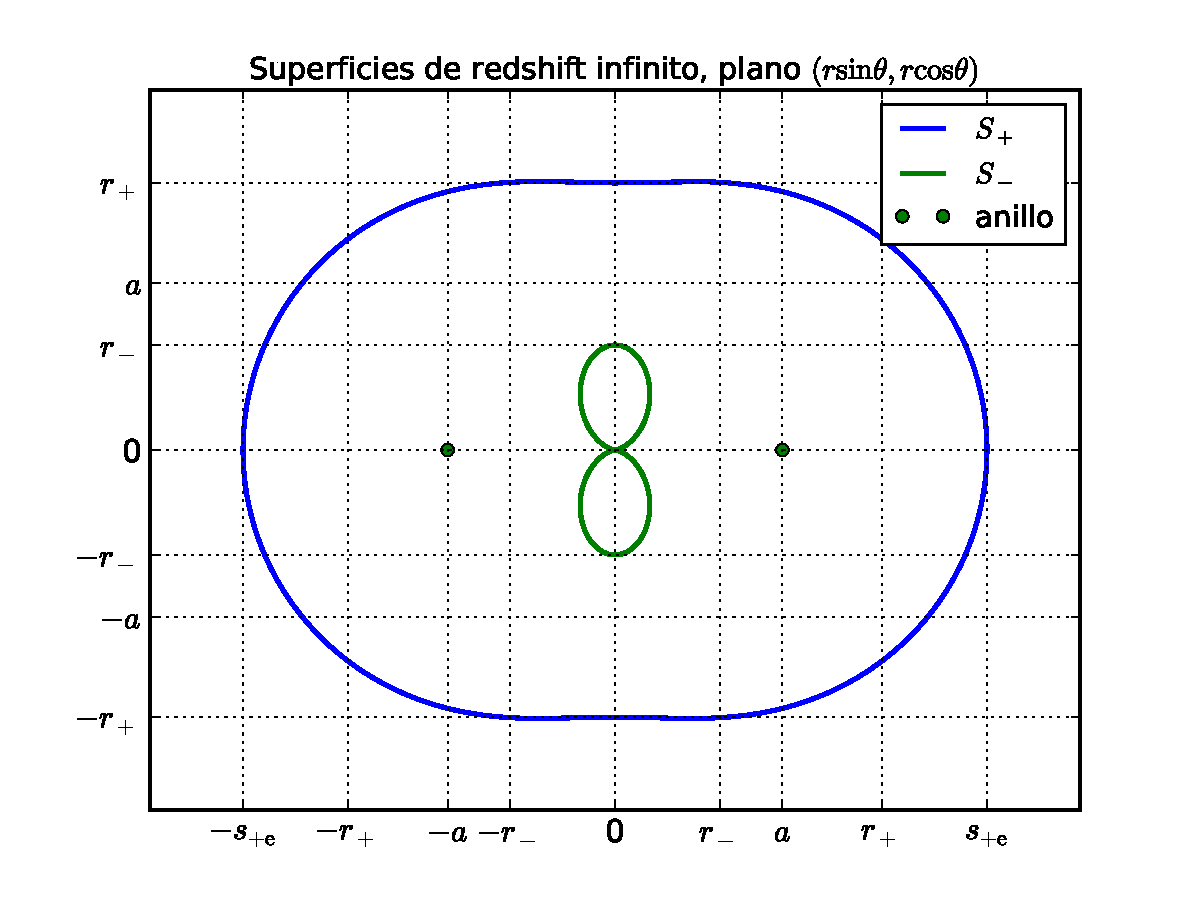
\includegraphics[height=7cm,angle=0]{fig/fig-superficies-1.pdf}
\caption{Superficies de redshift infinito. C'odigo Python \href{https://github.com/gfrubi/GR/blob/master/figuras-editables/fig-superficies-Kerr-01.py}{aqu\'i}.}
\label{fig:surface1}
\end{figure}
De \eqref{rsk} se observa que al hacer $a=0$, se obtiene lo ya sabido para la soluci\'on no rotante, donde $r_{S_{+}}$ coincide con el radio de
Schwarzschild $2m$ y el valor de $r_{S_{-}}$ con el de la singularidad.

Ahora, se buscar\'an superficies donde existan \textit{horizontes de eventos}. De \eqref{BL2} vemos que el horizonte estar'a ubicado en los puntos en los que $g_{rr}$ diverge, es decir, donde $\Delta$ se anula
\begin{equation}\label{grr}
g_{rr}=-\frac{\rho^2}{\Delta}\rightarrow -\infty \quad\Rightarrow\quad r^2-2mr+a^2=0.
\end{equation}
As\'i, los horizontes de eventos vienen dados por
\begin{equation}\label{horizontes}
\boxed{r_{\pm}=m\pm\sqrt{m^2-a^2}.}
\end{equation}
Note que estos horizontes existes s'olo si $a^2\leqslant m^2$. En el caso que $a^2>m^2$ se tiene que el campo gravitacional tiene una singularidad ``desnuda'' (debido a la no existencia de horizontes de eventos). La hip'otesis que esto no ocurre en la naturaleza es lo que se conoce como la \textit{Conjetura de Censura C\'osmica de Penrose}\footnote{Sir Roger Penrose (1931-) f\'isico-matem\'atico ingl\'es, \url{http://es.wikipedia.org/wiki/Roger_Penrose}.} que afirma que un colapso gravitacional que tiene condiciones iniciales bien comportadas nunca dar\'a origen a una singularidad desnuda. El agujero negro que tiene $a=m$ es llamado \textit{agujero negro maximalmente rotante}.\\

Luego, existen tres zonas (sin incluir la singualridad intr\'inseca) en las cuales la soluci\'on de Kerr es regular
\begin{equation}
\begin{aligned}
I&:\quad r_+<r<\infty\\
II&:\quad r_{-}<r<r_{+}\\
III&:\quad 0<r<r_{-}
\end{aligned}
\end{equation}

\begin{figure}[H]
 \centering
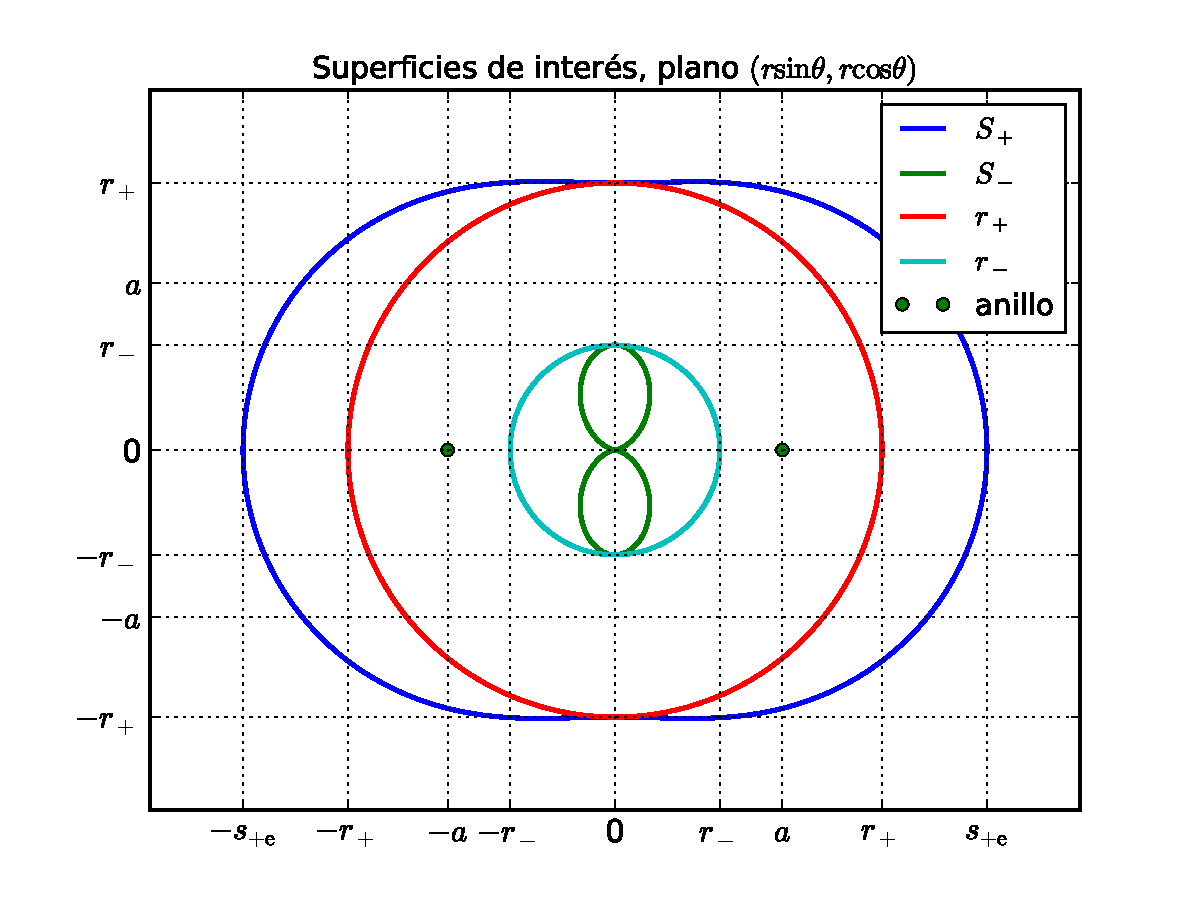
\includegraphics[height=7cm,angle=0]{fig/fig-superficies-2.pdf}
\caption{Horizontes y superficies de redshift infinito de la soluci\'on de Kerr.  C'odigo Python \href{https://github.com/gfrubi/GR/blob/master/figuras-editables/fig-superficies-Kerr-01.py}{aqu\'i}.}
\label{fig:surface2}
\end{figure}

Si $a=0$, entonces $r_{+}=2m$ y $r_{-}=0$, que tambi\'en coinciden con el radio de Schwarzschild y la singularidad intr\'inseca de ese caso. Se tiene que, como se mencion\'o anteriormente, en el caso de la soluci\'on de Schwarzschild $S_{+}$ coincide con el horizonte de eventos y $S_{-}$ con la singularidad en el origen.\\

Se define la \textit{Erg\'osfera} (del griego \textit{ergon} que significa trabajo) como la zona que existe entre la superficie de redshift infinito $S_{+}$ y el horizonte de eventos $r_{+}$(ver figura \ref{fig:surface2}), cuyas propiedades ser\'an analizadas m\'as adelante.\\

\begin{figure}[H]
 \centering
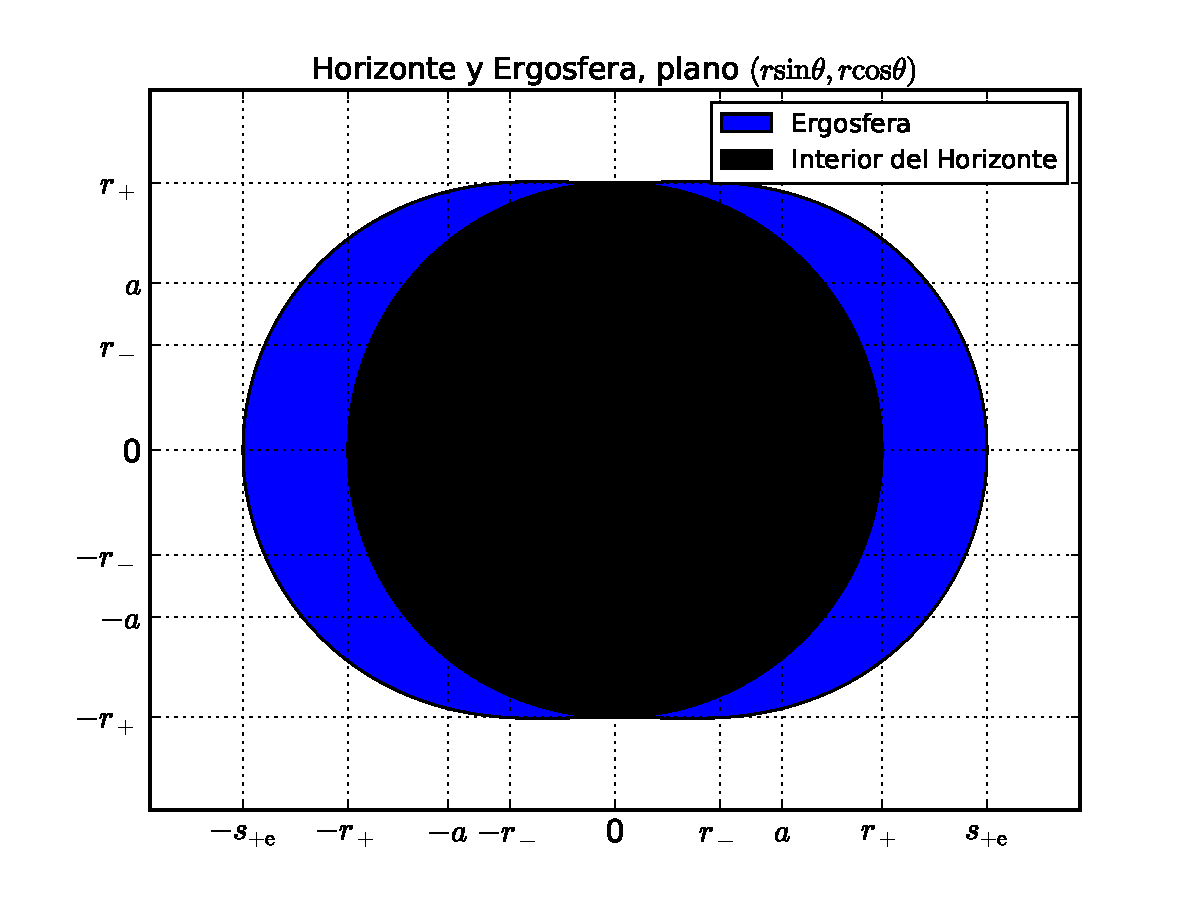
\includegraphics[height=7cm,angle=0]{fig/fig-superficies-3.pdf}
\caption{Horizonte de eventos y erg\'osfera de la soluci\'on de Kerr. C'odigo Python  \href{https://github.com/gfrubi/GR/blob/master/figuras-editables/fig-superficies-Kerr-01.py}{aqu\'i}.}
\label{fig:surface3}
\end{figure}

\subsection{Geod\'esicas tipo luz}

A diferencia de la soluci\'on de Schwarzschild en este caso no existen geod\'esicas nulas radiales, ya que no hay simetr\'ia esf\'erica, pero s\'i es posible encontrar geod\'esicas nulas (de una part\'icula tipo luz) a partir del hecho que esta soluci\'on es axialmente sim\'etrica, es decir, buscaremos geod\'esicas con la condici\'on $\theta=\rm cte$. As\'i
\begin{equation}
\dot{\theta}=0,\qquad ds^2=0.
\end{equation}

El punto sobre la coordenada denota la derivada con respecto a un par\'ametro af\'in $\lambda$. Lo siguiente es resolver la ecuaciones de Euler-Lagrange para este caso. Se sabe que el lagrangiano de una part\'icula tiene la siguiente forma
\begin{equation} \label{lagrange1}
L=\alpha\sqrt{-g_{\mu \nu}\dot{x}^{\mu}\dot{x}^{\nu}}.
\end{equation}
 
Donde $\alpha$ es una constante con dimensiones de momentum lineal y $g_{\mu \nu}$ viene dada por \eqref{BL}. Pero, si se utiliza un par\'ametro af\'in entonces se puede demostrar que el lagrangiano dado por
\begin{equation} \label{lagrange2}
\tilde{L}=-\beta g_{\mu \nu}\dot{x}^{\mu}\dot{x}^{\nu}.
\end{equation}
 
conduce a las mismas ecuaciones de Euler-Lagrange que \eqref{lagrange1}, donde $\beta$ una constante que dimensionaliza el lagrangiano. Luego, se utilizar\'a por simplicidad \eqref{lagrange2} para derivar las ecuaciones de movimiento. La funci\'on que se utilizar\'a para obtener las ecuaciones de movimiento es
\begin{equation}\label{lagrangeano1}
\tilde{L}=-\beta\left[\frac{\Delta}{\rho^2}(c\dot{t}-a\sen^2\theta \dot{\varphi})^2-\frac{\sen^2\theta}{\rho^2}\left[(r^2+a^2)\dot{\varphi}-ac\dot{t} \right]^2-\frac{\rho^2}{\Delta}\dot{r}^2\right].
\end{equation}

Las ecuaciones de Euler-Lagrange vienen dadas por
\begin{equation}\label{el}
\frac{\partial \tilde{L}}{\partial x^{\mu}}-\frac{d}{d\lambda}\left(\frac{\partial \tilde{L}}{\partial \dot{x}^{\mu}} \right)=0.
\end{equation}

Utilizando $x^0=ct$ en \eqref{el}, se obtiene la primera ecuaci\'on de movimiento:
\begin{equation}\label{elt}
\frac{\partial}{\partial c\dot{t}}\left(g_{\mu \nu}\dot{x}^{\mu}\dot{x}^{\nu}\right)=l.
\end{equation}
 
Donde $l$ es una constante de integraci\'on. Desarrollando \eqref{elt}, se tiene lo siguiente:
\begin{equation}\label{11}
\frac{\Delta}{\rho^2}\left(c\dot{t}-a\sen^2 \theta \dot{\varphi}\right)+\frac{a\sen^2 \theta}{\rho^2}\left[(r^2+a^2)\dot{\varphi}-ac\dot{t} \right]=l.
\end{equation} 
 
 Ahora se buscar\'a la ecuaci\'on de movimiento correspondiente a $x^3=\varphi$, nuevamente de \eqref{el} se obtiene la siguiente ecuaci\'on de movimiento
 \begin{equation}\label{elp}
 \frac{\partial}{\partial \dot{\varphi}}\left(g_{\mu \nu}\dot{x}^{\mu}\dot{x}^{\nu}\right)=n,
 \end{equation}
 
donde $n$ tambi\'en es una constante de movimiento.\\

De \eqref{elp} se tiene que
\begin{equation}\label{22}
\frac{a\Delta \sen^2 \theta}{\rho^2}\left(c\dot{t}-a\sen^2 \theta \dot{\varphi}\right)+\frac{(r^2+a^2)\sen^2 \theta}{\rho^2}\left[(r^2+a^2)\dot{\varphi}-ac\dot{t} \right]=n.
\end{equation}
 
Usando el hecho que $ds^2=0$ y la expresi\'on \eqref{BL}, se tiene lo siguiente:
\begin{equation}\label{33}
\frac{\Delta}{\rho^2}(c\dot{t}-a\sen^2\theta \dot{\varphi})^2-\frac{\sen^2\theta}{\rho^2}\left[(r^2+a^2)\dot{\varphi}-ac\dot{t} \right]^2-\frac{\rho^2}{\Delta}\dot{r}^2=0.
\end{equation} 
 
Por \'ultimo utilizando $x^2=\theta$ y de \eqref{el}, se tiene que la ecuaci\'on de movimiento asociada a esta coordenada es
\begin{equation}
\frac{\partial }{\partial \theta}\left(g_{\mu \nu}\dot{x}^{\mu}\dot{x}^{\nu} \right)=0.
\end{equation} 

Desarrollando esta \'ultima expresi\'on se obtiene que
\begin{equation}\label{44}
\frac{a^2\Delta}{\rho^4}\left(c\dot{t}-a\sen^2 \theta \dot{\varphi} \right)^2-\frac{2a\Delta \dot{\varphi}}{\rho^2}\left(c\dot{t}-a\sen^2 \theta \dot{\varphi} \right)-\frac{(r^2+a^2)}{\rho^4}\left[(r^2+a^2)\dot{\varphi}-ac\dot{t} \right]^2+\frac{a^2\dot{r}^2}{\Delta}=0.
\end{equation}
 
Se obseva que s\'olo existen 3 inc\'ognitas ($\dot{t}$, $\dot{r}$ y $\dot{\varphi}$) y 4 ecuaciones, a saber, \eqref{11}, \eqref{22}, \eqref{33} y \eqref{44}. Por lo tanto, debe existir una expresi\'on que relacione los t\'erminos constantes $l$ y $n$. De \eqref{11} y \eqref{22} se obtienen las siguientes relaciones:
\begin{equation}\label{55}
\sen^2\theta \left[(r^2+a^2)\dot{\varphi}-ac\dot{t} \right]=(n-al\sen^2\theta),
\end{equation}
 
\begin{equation}\label{66}
\Delta(c\dot{t}-a\sen^2\theta\dot{\varphi})=\left[(r^2+a^2)l-an\right].
\end{equation}
 
De estas \'ultimas se puede despejar $\dot{\varphi}$, que viene dado por
\begin{equation}\label{77}
\dot{\varphi}=\frac{1}{\rho^2\sen^2\theta}(n-al\sen^2\theta)+\frac{a}{\Delta}\left[(r^2+a^2)l-an\right].
\end{equation}
 
 Por otro lado, de \eqref{33} y \eqref{44} se tiene que
 \begin{equation}\label{88}
 \begin{aligned}
 \frac{2a^2\Delta}{\rho^4}(n-al\sen^2\theta)^2-\frac{2a\Delta \dot{\varphi}}{\rho^2}(n-al\sen^2\theta)&-\frac{(r^2+a^2)}{\rho^4}\left[(r^2+a^2)l-an\right]^2\\
 &-\frac{a^2\sen^2\theta}{\rho^4}\left[(r^2+a^2)l-an\right]^2=0.\\
 \end{aligned}
 \end{equation}
 
 Reemplazando \eqref{55}, \eqref{66} y \eqref{77} en \eqref{88} se obtiene la ecuaci\'on que relaciona a $l$ y $n$:
 \begin{equation}
 (n+al\sen^2 \theta)(n-al\sen^2 \theta)=0.
 \end{equation}
 
Se escoger\'a la condici\'on $n-al\sen^2\theta=0$, que si es utilizada en \eqref{55} se tiene que
\begin{equation}\label{dott}
c\dot{t}=\frac{(r^2+a^2)}{a}\dot{\varphi}.
\end{equation}

Reemplazando \eqref{dott} en \eqref{11}, se puede despejar una expresi\'on para $\dot{\varphi}$
\begin{equation}\label{dotvar}
\dot{\varphi}=\frac{al}{\Delta}.
\end{equation}

As\'i, la ecuaci\'on para $c\dot{t}$ es
\begin{equation}\label{dott2}
c\dot{t}=\frac{(r^2+a^2)l}{\Delta}.
\end{equation}

Utilizando \eqref{dott} y \eqref{dotvar} en \eqref{33} se obtiene que
\begin{equation}
\dot{r}=\pm l.
\end{equation}

Luego, $r=\pm l\lambda+c$, donde $c$ es una constante, lo que entrega la libertad de elegir a $r$ como el par\'ametro af\'in a lo largo de cada geod\'esica, escogiendo en part\'icular $r=+l$, se tiene de \eqref{dotvar} que
\begin{equation}\label{var1}
\frac{d \varphi}{dr}=\frac{\dot{\varphi}}{\dot{r}}=\frac{a}{\Delta}.
\end{equation}

Por otra parte de \eqref{dott2} se tiene que
\begin{equation}\label{t}
\frac{d(ct)}{dr}=\frac{c\dot{t}}{\dot{r}}=\frac{r^2+a^2}{\Delta}.
\end{equation}
 
Estas ecuaciones pueden ser integradas f\'acilmente. De \eqref{var1}  se tiene lo siguiente 
\begin{equation}
\begin{aligned}
\varphi(r)&=\int_{r_0}^r \frac{adr'}{\Delta} + \varphi_0\\
&=a\int_{r_0}^r\frac{dr'}{(r'-r_+)(r'-r_-)} + \varphi_0\\
&=\frac{a}{r_+-r_-}\int_{0}^r\left(\frac{1}{r'-r_+} - \frac{1}{r'-r_-} \right)dr'+\varphi_0\\
&=\frac{a}{r_+-r_-}\ln \left|\left(\frac{r-r_+}{r-r_-}\right)\left(\frac{r_0-r_-}{r_0-r_+} \right)\right| + \varphi_0.
\end{aligned}
\end{equation}
 
 Utilizando \eqref{horizontes} se tiene que 
 $$r_+-r_-=2\sqrt{m^2-a^2}.$$ 
 
 Considerando que $a^2<m^2$, se ecuentra que la expresi\'on para $\varphi$ como funci\'on de la coordenada $r$ de una curva que pasa por las coordenadas $(r_0,\varphi_0)$ es
\begin{equation}\label{congphi}
\boxed{\varphi(r)=\frac{a}{2\sqrt{m^2-a^2}}\ln \left|\left(\frac{r-r_+}{r-r_-}\right)\left(\frac{r_0-r_-}{r_0-r_+} \right)\right| + \varphi_0.}
\end{equation}  

De \eqref{t} se tiene que
\begin{equation}
\begin{aligned}
ct&=\int_{r_0}^r\frac{r'^2+a^2}{\Delta}dr'+ct_0\\
&=\int_{r_0}^r \frac{r'^2dr'}{(r'-r_+)(r'-r_-)}+a^2\int_{r_0}^r\frac{dr'}{(r'-r_+)(r'-r_-)}+ct_0.\\
\end{aligned}
\end{equation}

Se tiene adem\'as que
\begin{equation}
\int \frac{r^2dr}{(r-r_+)(r-r_-)}=r+\frac{r_{+}^2 \ln |r-r_+|}{r_+-r_-}-\frac{r_{-}^2\ln |r-r_-|}{r_+-r_-}.
\end{equation}

Luego
\begin{equation}
ct=r-r_0+\frac{(r_+^2+a^2)}{r_+-r_-}\ln\left|\frac{r-r_+}{r_0-r_+}\right|-\frac{(r_-^2+a^2)}{r_+-r_-}\ln \left|\frac{r-r_-}{r_0-r_-}\right|+ct_0.
\end{equation}

Al igual que en el c\'alculo de la expresi\'on para $\varphi$ se utiliza \eqref{horizontes} para encontrar lo siguiente
\begin{equation*}
r_{\pm}^2=m^2+\pm 2m\sqrt{m^2-a^2}+m^2-a^2.
\end{equation*}

As\'i, la expresi\'on buscada para $t$ como funci\'on de la coordenada $r$ de una curva que pasa por la coordenadas $(ct_0,r_0)$ es
\begin{equation}\label{congt}
\boxed{ct(r)=r-r_0+\left(m+\frac{m^2}{\sqrt{m^2-a^2}} \right)\ln\left|\frac{r-r_+}{r_0-r_+}\right|+\left(m-\frac{m^2}{\sqrt{m^2-a^2}} \right)\ln \left|\frac{r-r_-}{r_0-r_-}\right|+ct_0 .}
\end{equation}

Tal como se oberva en la figura \ref{fig:delta}, se tiene que $\Delta$ es positivo en las regiones $I$ y $III$, mientras que es negativo en la regi\'on $II$.

\begin{figure}[H]
 \centering
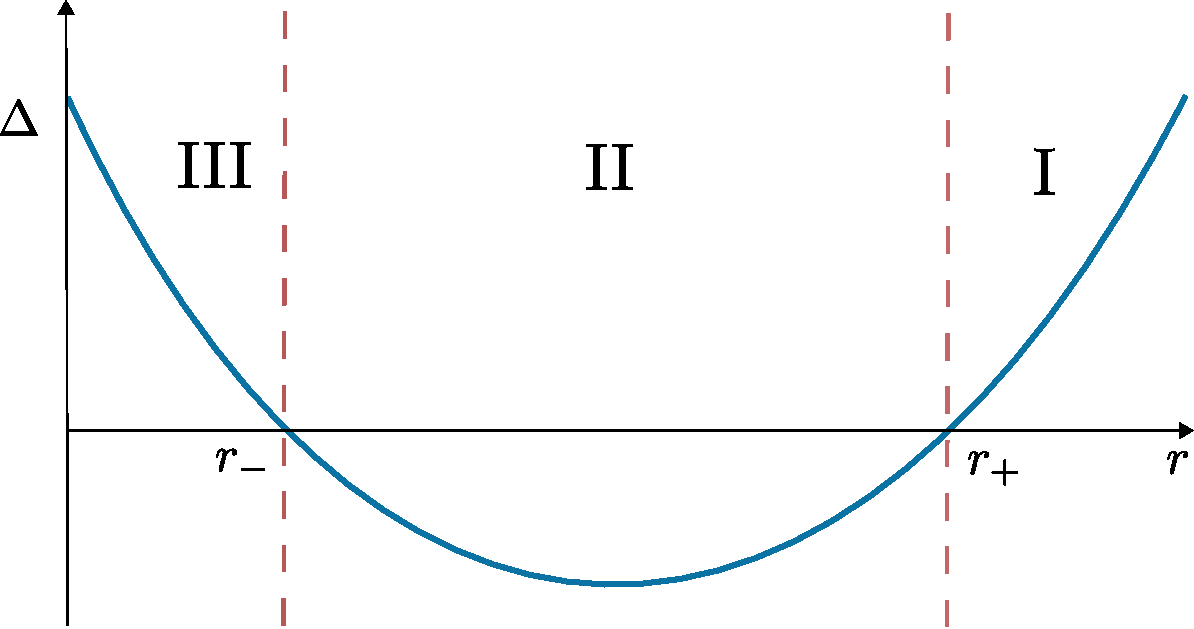
\includegraphics[height=5cm,angle=0]{fig/fig-delta.pdf}
\caption{Funci\'on $\Delta$ versus coordenada $r$}
\label{fig:delta}
\end{figure}

Como $\Delta >0$ en $I$ entonces $dr/dt>0$, as\'i las curvas son salientes en esta regi\'on con esta elecci\'on de signo en $\dot{r}$ ($\dot{r}=+l$),  a este conjunto de curvas (congruencia) se le llama \textit{congruencia principal de las geod\'esicas salientes tipo luz}. Mientras que si la elecci\'on es con signo negativo en $\dot{r}$, entonces $dr/dt<0$, donde esta congruencia es llamada \textit{congruencia principal de las geod\'esicas entrantes tipo luz}, cabe destacar que este caso es equivalente a hacer el cambio de signo simult\'aneamente en $ct$ y $\varphi$
\begin{equation}
\frac{dr}{dt}<0 \quad \Longleftrightarrow \quad ct \rightarrow -ct \quad \wedge \quad \varphi \rightarrow -\varphi .
\end{equation}

Por lo tanto, la expresi\'on para estas curvas es
\begin{equation}
\begin{aligned}
\varphi(r)&=-\frac{a}{2\sqrt{m^2-a^2}}\ln \left|\left(\frac{r-r_+}{r-r_-}\right)\left(\frac{r_0-r_-}{r_0-r_+} \right)\right| + \varphi_0 ,\\
ct(r)&=r_0-r-\left(m+\frac{m^2}{\sqrt{m^2-a^2}} \right)\ln\left|\frac{r-r_+}{r_0-r_+}\right|-\left(m-\frac{m^2}{\sqrt{m^2-a^2}} \right)\ln \left|\frac{r-r_-}{r_0-r_-}\right|+ct_0.\\
\end{aligned}
\end{equation}

Al hacer $a=0$ en \eqref{congphi} y \eqref{congt} se obtiene lo siguiente
\begin{equation}
\begin{aligned}
\varphi &=\varphi_0 ,\\
ct&=r-r_0+2m\ln|r-2m|+ct_0,\\
\end{aligned}
\end{equation}
que corresponden a las congruencias salientes, de la soluci\'on de Schwarzschild dadas en \eqref{rtfs} para el caso de part\'iculas tipo luz moviendose radialmente.\\

\subsection{Diagrama Espacio-Temporal}

Al representar gr\'aficamente la expresi\'on \eqref{congt} se obtiene el llamado diagrama espacio-temporal de los conos de luz (figura \ref{fig:conos1}), donde se observa que a medida que los conos se aproximan al horizonte de eventos $r_+$ en la regi\'on $I$ \'estos se empiezan a estrechar, hasta que la coordenada $t$ diverge, como es de esperar, ya que $r=r_+$ es una singularidad de las coordenadas. \'Esta puede ser removida al igual que en el caso de la soluci\'on de Schwarschild con un buen cambio de coordenadas.

 \begin{figure}[H]
 \centering
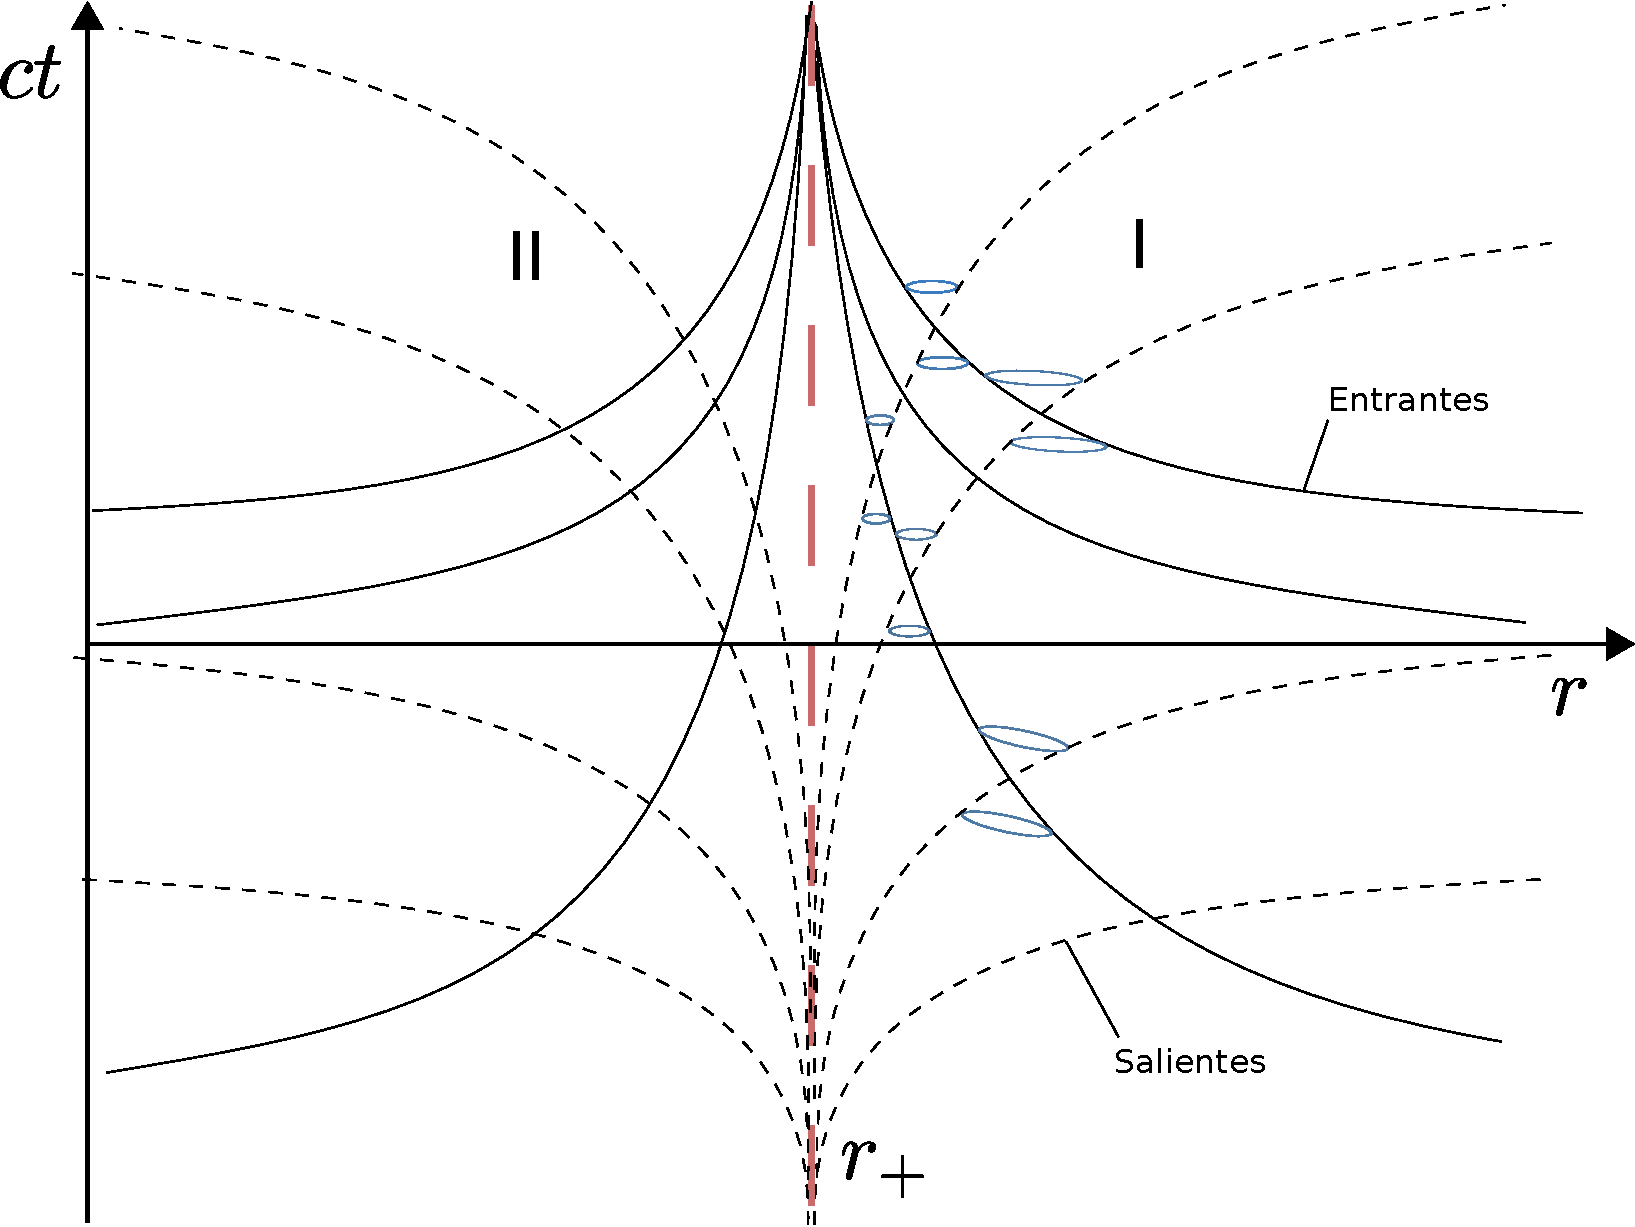
\includegraphics[height=6cm,angle=0]{fig/fig-conos1.pdf}
\caption{Diagrama espacio-tiempo en la vecindad de $r_+$}
\label{fig:conos1}
\end{figure}
  
Con ese prop\'osito se buscar\'a un an\'alogo al sistema de coordenadas de Eddington-Finkelstein utilizado en la soluci\'on de Schwarzschild. 

\subsubsection{Coordenadas de Eddington-Finkelstein} 

En el caso de la m\'etrica de Schwarzschild para extender las congruencias entrantes a trav\'es del horizonte de eventos $r=r_+$ se hac\'ia que las geod\'esicas tuvieran pendiente $-1$ en un diagrama espacio-tiempo durante todo su recorrido hasta llegar a la singularidad geom\'etrica, es decir, para encontrar las coordenadas de Eddington-Finkelstein $(c\bar{t},r,\varphi,\theta)$ se utiliz\'o la siguiente condici\'on: 
\begin{equation}
\frac{d(ct)}{dr}=-1 \quad \Rightarrow \quad d(ct)=-dr,
\end{equation}

Donde las coordenadas $(\varphi,\theta )$ eran constantes, esto es
\begin{equation}
d\varphi=0, \qquad d\theta=0 .
\end{equation}

En este caso se utilizar\'an las mismas condiciones, pero sobre las relaciones ya conocidas \eqref{t} y \eqref{var1}, utilizando $\dot{r}=-l$, as\'i
\begin{equation}
\begin{aligned}
d(ct)&=-\frac{r^2+a^2}{\Delta}dr,\\
d \varphi&=-\frac{a}{\Delta}dr,\\
\end{aligned}
\end{equation}

tal que
\begin{equation}
d\left(c\bar{t}\right)=-dr, \qquad d\bar{\varphi}=0 .
\end{equation}

Es f\'acil verificar que la transformaci\'on entre coordenadas buscada, en su forma diferencial, viene dada por
\begin{equation}
\begin{aligned}
d\left(c\bar{t}\right)&=d(ct)+\frac{2mr}{\Delta}dr,\\
d\bar{\varphi}&=d	\varphi+\frac{a}{\Delta}dr.\\
\end{aligned}
\end{equation}

Por lo tanto, las congruencias entrantes de las geod\'esicas nulas  en el sistema de coordenadas de Eddington-Finkelstein vienen dadas por
\begin{equation}
\begin{aligned}
c\bar{t}&=r_0-r+ct_0,\\
\bar{\varphi}&=\varphi_0.\\
\end{aligned}
\end{equation}

\'Estas se pueden ver en la figura \ref{fig:conos2}, donde la trayectoria para las geod\'esicas entrantes no son alteradas por los horizontes de eventos, no as\'i con las congruencias salientes, donde los valores de $ct$ y $\phi$ divergen en estos puntos ($r_-,r_+$).\\
\begin{figure}[H]
 \centering
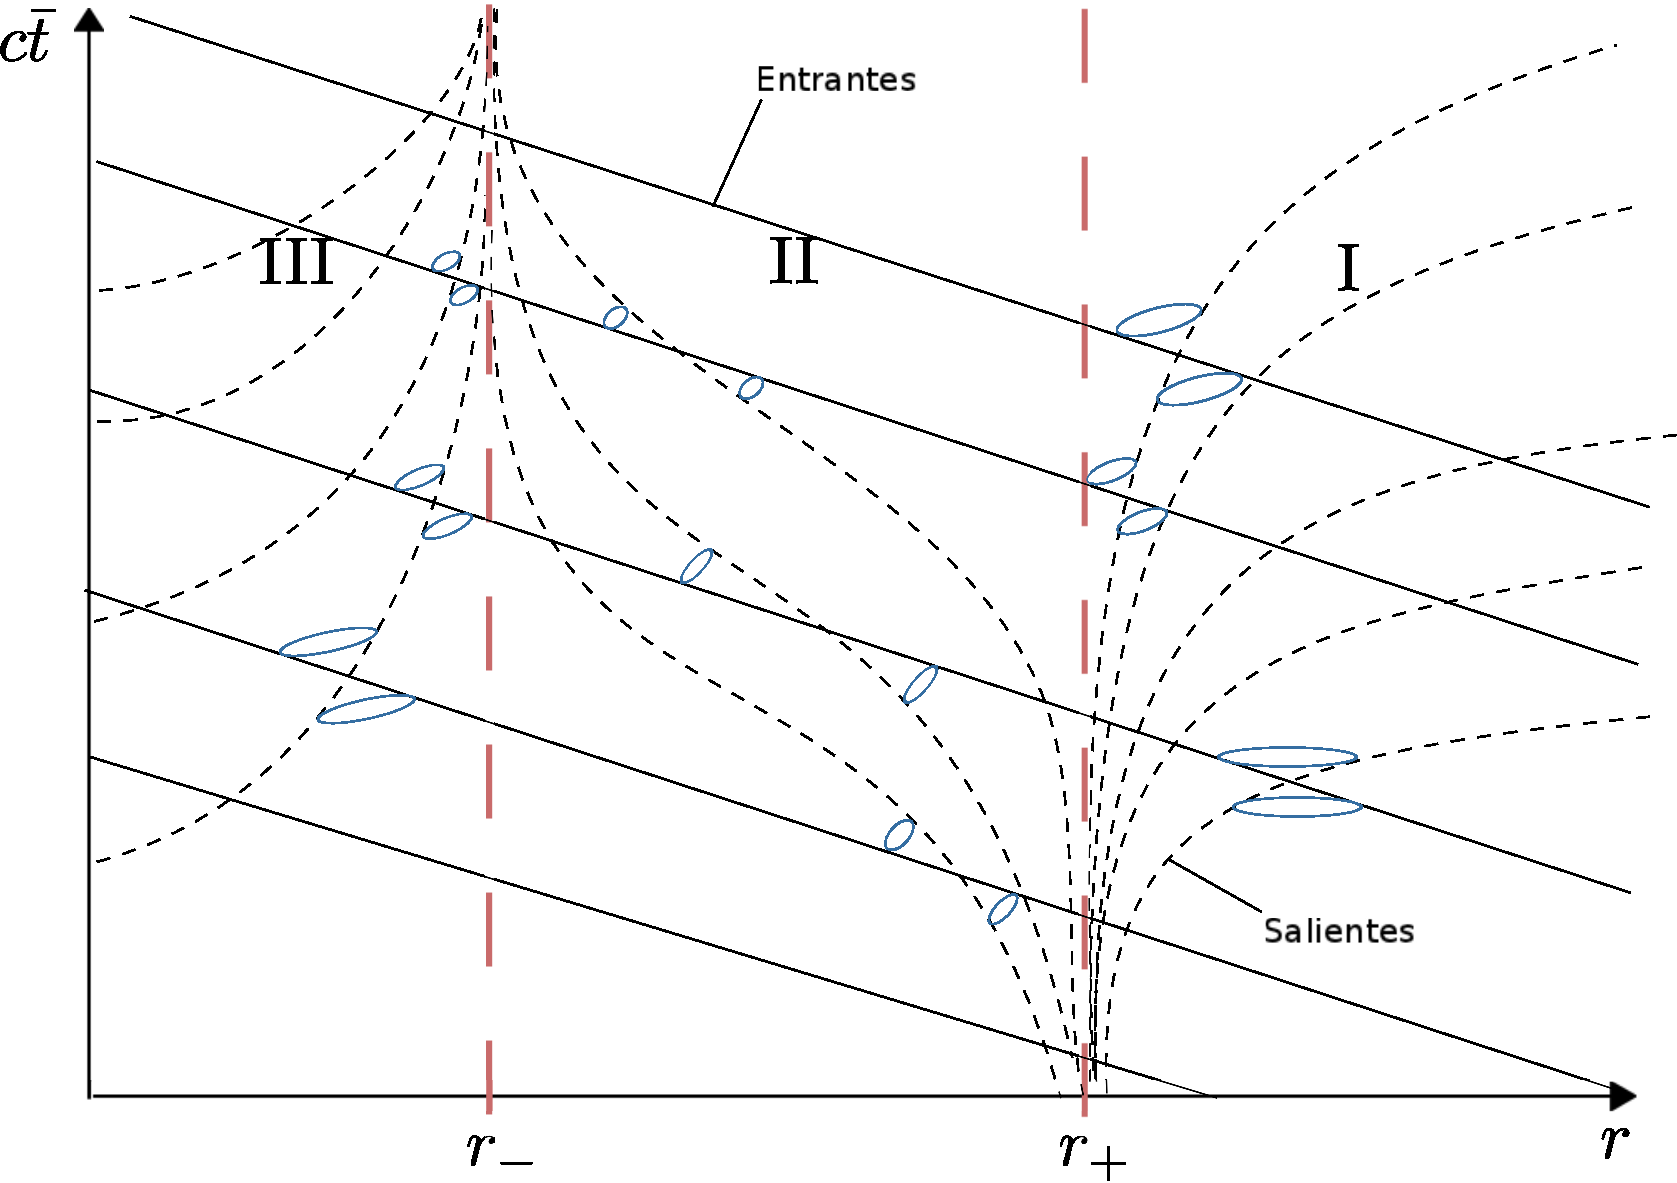
\includegraphics[height=6cm,angle=0]{fig/fig-conos2.pdf}
\caption{Diagrama de espacio tiempo en coordenadas de Eddington-Finkelstein.}
\label{fig:conos2}
\end{figure}

\subsection{L\'imite Estacionario y Observadores Estacionarios}

Al analizar la m\'etrica de Schwarzschild fue necesario utilizar observadores est\'aticos en el infinito, para estudiar la m\'etrica de Kerr se generaliza este concepto utilizando los llamados \textit{Observadores Estacionarios} que se eligen de tal forma que $r$ y $\theta$ permanezcan fijos
y que roten en torno al eje de giro del agujero negro con velocidad angular constante $\Omega$ dada por
\begin{equation}
\Omega=\frac{d\varphi}{dt}=c\frac{u^{\varphi}}{u^{0}},
\end{equation}
donde $u^{\mu}=dx^{\mu}/d\tau$ con $\tau$ el tiempo propio. Utilizando el hecho que el observador tiene una l\'inea de mundo tipo tiempo $(u^{\mu}u_{\mu}=c^2)$ entonces se debe cumplir que
\begin{equation}\label{cuadrados}
\left(u^{0}\right)^2\left[g_{\varphi \varphi}\frac{\Omega^2}{c^2}+2g_{\varphi 0}\frac{\Omega}{c} +g_{00}\right]=c^2, \qquad \theta=\frac{\pi}{2}.
\end{equation}

As\'i la expresi\'on entre corchetes cuadrados debe ser positiva. Debido  a que esa funci\'on tiene concavidad hacia abajo ($g_{\varphi \varphi}<0$), entonces 
\begin{equation}
\Omega_{-}<\Omega <\Omega_{+},
\end{equation}
donde $\Omega_{\pm}$ son la ra\'ices de la expresi\'on entre corchetes cuadrados en \eqref{cuadrados}
\begin{equation}\label{roots}
\Omega_{\pm}= c\left[ \frac{-g_{0\varphi}\pm\sqrt{g_{0\varphi}^2-g_{00}g_{\varphi \varphi}}}{g_{\varphi \varphi}} \right].
\end{equation}

Utilizando \eqref{BL2} notamos que $\Omega_{-}=0$ cuando $g_{00}=r^2-2mr+a^2\cos^2 \theta=0$, cuya soluci\'on (respetando que $r_+<r$) es justamente la superficie de redshift infinito $S_{+}$ que viene dada por el radio
\begin{equation}
r_{s_+}=m+\sqrt{m^2-a^2\cos^2\theta}.
\end{equation}

En el caso que $r_+<r<r_{s_+}$ la velocidad angular $\Omega$ siempre ser\'a postivo ya que en ese caso $\Omega_{-}>0$, que viene del hecho que $g_{00}>0$ (coordenada $ct$ es tipo tiempo). Por lo tanto, en este rango no pueden existir observadores est\'aticos (es decir con $\Omega=0$). As\'i, s\'olo en el caso en que $r=r_{s_+}$ se tiene que $\Omega=0$, raz\'on por la cual se le llama \textit{L\'imite Est\'atico}.\\

De \eqref{roots} se observa que los observadores estacionarios no existen si $g_{0\varphi}^2-g_{00}g_{\varphi \varphi}<0$, lo que se traduce en que $\Delta <0$, ya que
\begin{equation}
(r-r_-)(r-r_+)<0.
\end{equation}
As\'i, los observadores estacionarios existen s\'olo cuando $r>r_+$ que viene a ser la generalizaci\'on del hecho que los observadores est\'aticos no existen dentro del horizonte de eventos en la soluci\'on de Schwarzschild.\\

\subsubsection{Estructura de los Conos de Luz en la Erg\'osfera}

Se consideran ahora curvas de part\'iculas tipo luz que tienen las coordenadas $r$ y $\theta$ fijas $(dr=d\theta=0)$ (no son geod\'esicas), es decir, part\'iculas que inicialmente estaban obligadas a orbitar la fuente con esta condici\'on de \eqref{BL} se obtiene que
\begin{equation}
\frac{\Delta}{\rho^2}(cdt-a\sen^2\theta d\varphi)^2-\frac{\sen^2\theta}{\rho^2}\left[(r^2+a^2)d\varphi-acdt \right]^2=0,
\end{equation}

de donde se tiene que 
\begin{equation}\label{dphidt}
\left( \frac{d\varphi}{dt} \right) _{\pm}=\frac{ac\sen \theta \pm c\sqrt{\Delta}}{(r^2+a^2)\sen\theta \pm a\sqrt{\Delta}\sen^2\theta}.
\end{equation}

En el caso de elegir la soluci\'on positiva en \eqref{dphidt} entonces  $d\varphi/dt >0$, con lo cual la part\'icula gira en el mismo sentido de la fuente. Ahora la pregunta es, para qu\'e caso  $d\varphi/dt \leqslant 0$, es decir, que la part\'icula gira en sentido contrario o parece estacionaria en estas coordenadas.\\

Si se parte con la condici\'on $r> r_{+}$ en la soluci\'on negativa de \eqref{dphidt} se puede concluir f\'acilmente que el denominador de \eqref{dphidt} es positivo
\begin{equation}
(r^2+a^2)\sen\theta - a\sqrt{\Delta}\sen^2\theta >0.
\end{equation}

Luego, el sentido de rotaci\'on queda inmediatamente ligado al numerador de \eqref{dphidt}
\begin{equation} \label{numerador}
\frac{d\varphi}{dt}  \leqslant   0 \quad  \Leftrightarrow \quad  a\sen \theta - \sqrt{\Delta} \leqslant 0.
\end{equation} 

Desarrollando en \eqref{numerador} la condici\'on impuesta en el numerador, podemos escribir
\begin{equation}
\begin{aligned}
a^2\sen^2 \theta &\leqslant \Delta ,\\
 a^2\sen^2 \theta &\leqslant r^2-2mr+a^2 , \\
 0 &\leqslant r^2-2mr+a^2\cos^2 \theta ,\\
 0 &\leqslant (r-r_{s_{+}})(r-r_{s_{-}}).\\
\end{aligned}
\end{equation}

Como $r>r_{+}$ entonces $r>r_{s_-}$, luego la condici\'on buscada para que \eqref{dphidt} sea menor o igual que cero es que
\begin{equation}
r\geqslant r_{s_+}.
\end{equation}

Analizando este resultado, se tiene que si la part\'icula se encuentra sobre la superficie $S_+$, entonces \'esta parece estar estacionaria (para un observador estacionario en el infinito). En cambio m\'as all\'a de la supeficie dada, las part'iculas luminosas en el r\'egimen impuesto recorren las curvas en sentido inverso a la rotaci\'on de la fuente, no as\'i dentro de la erg\'osfera, donde las part\'iculas orientan su cono luz en la direcci\'on del giro de la fuente.\\

\section{Extracci\'on de Energ\'ia de una Agujero Negro Rotante}

\subsection{Geod\'esicas tipo tiempo}

En este caso se calcular\'an las geod\'esicas de part\'iculas en movimiento en el plano ecuatorial $\theta=\pi/2$. Para resolver el caso general se puede utilizar una forma descubierta por B. Carter\footnote{Brandon Carter (1942) f\'isico te\'orico australiano \url{http://en.wikipedia.org/wiki/Brandon_Carter}.} (ver $[41]$) donde utilizan el m\'etodo de Hamilton-Jacobi.

Utilizando la funci\'on lagrangeana proporcional a la dada en \eqref{lagrangeano1}, se tiene que
\begin{equation}\label{lagrangeano2}
\tilde{L}=\frac{1}{2}g_{\mu \nu} \dot{x}^{\mu} \dot{x}^{\nu}=\frac{1}{2}\left[\left(1-\frac{2m}{r}\right)c^2\dot{t}^2-\frac{r^2}{\Delta}\dot{r}^2-\left(r^2+a^2+\frac{2ma^2}{r}\right)\dot{\varphi}^2
+\frac{4am}{r}\dot{\varphi}(c\dot{t}) \right],
\end{equation}
con $\dot{x}^{\mu}=dx^{\mu}/d \lambda$ y $\lambda$ es un par\'ametro af\'in. Por conveniencia elegimos $\lambda=\tau/m_0$, donde $m_0$ es la masa de la part\'icula movi\'endose en este campo gravitacional y $\tau$ su tiempo propio. Tal como se puede observar en \eqref{lagrangeano2} este lagrangiano no depende expl'icitamente de las coordenadas $ct$ y $\varphi$, por lo que existen dos constantes de movimiento\footnote{donde $E$ es la energ\'ia de la part\'icula y $L$ su momentum angular.}, a saber
\begin{equation}
\begin{aligned}
p_{t}&=\frac{\partial \tilde{L}}{\partial(c\dot{t})}=\left(1-\frac{2m}{r}\right)c\dot{t}+\frac{2am\dot{\varphi}}{r}:=\frac{E}{c},\\ 
p_{\varphi}&=\frac{\partial \tilde{L}}{\partial \dot{\varphi}}=\frac{2am}{r}c\dot{t}-\left(r^2+a^2+\frac{2ma^2}{r}\right)\dot{\varphi}:=-L.\\
\end{aligned}
\end{equation}

Despejando $c\dot{t}$ y $\dot{\varphi}$, de estas ecuaciones se obtiene que
\begin{equation}
\begin{aligned}
c\dot{t}&=\frac{(r^3+a^2r+2ma^2)E/c-2amL}{r\Delta},\\ \label{dottdotphi}
\dot{\varphi}&=\frac{(r-2m)L+2amE/c}{r\Delta}.\\
\end{aligned}
\end{equation}

De la identidad $g_{\mu \nu}p^{\mu} p^{\nu}=g_{\mu \nu}\dot{x}^{\mu}\dot{x}^{\nu}=m_0^2c^2$, se tiene que 
\begin{equation}\label{pp=m2c2}
\left[\left(1-\frac{2m}{r}\right)c^2\dot{t}^2-\frac{r^2}{\Delta}\dot{r}^2-\left(r^2+a^2+\frac{2ma^2}{r}\right)\dot{\varphi}^2
+\frac{4am}{r}\dot{\varphi}(c\dot{t}) \right]=m_0^2c^2,
\end{equation}
de donde podemos despejar $\dot{r}^2$:
\begin{equation}\label{dotr}
\frac{r^2}{\Delta}\dot{r}^2=\left(1-\frac{2m}{r}\right)c^2\dot{t}^2-\left(r^2+a^2+\frac{2ma^2}{r}\right)\dot{\varphi}^2
+\frac{4am}{r}\dot{\varphi}(c\dot{t}) -m_0^2c^2.
\end{equation}

Reemplazando \eqref{dottdotphi} en \eqref{dotr}, obtenemos
\begin{equation}
\frac{r^2}{\Delta}\dot{r}^2=\left( r^3+a^2r+2ma^2\right)\frac{E^2}{c^2r\Delta}-4am\frac{EL}{cr\Delta}-\left(r-2m\right)\frac{L^2}{r\Delta}-m_0^2c^2.
\end{equation}

Por lo tanto,
\begin{equation}\label{dotr2}
r^3\dot{r}^2=\left( r^3+a^2r+2ma^2\right)\frac{E^2}{c^2}-4am\frac{E}{c}L-\left(r-2m\right)L^2-m_0^2c^2r\Delta .
\end{equation}

Definimos la funci\'on
\begin{equation}\label{R}
R(E,L,r):=\left( r^3+a^2r+2ma^2\right)\frac{E^2}{c^2}-4am\frac{E}{c}L-\left(r-2m\right)L^2-m_0^2c^2r\Delta,
\end{equation}
de modo que \eqref{dotr2} adopta la forma:
\begin{equation}
r^3\left(\frac{dr}{d\lambda}\right)^2=R(E,L,r).
\end{equation}

En el caso de que la \'orbita de la part\'icula sea una circunsferencia, $\dot{r}=0$ y $\ddot{r}=0$, lo que require que 
\begin{equation}
R=0, \qquad \frac{\partial R}{\partial r}=0.
\end{equation}

Con estas condiciones se pueden encontrar los valores de $E$ y $L$ para el caso de una \'orbita circular:
\begin{equation}
\frac{E}{m_0c^2}=\frac{r^2-2mr\pm a\sqrt{mr}}{r\left(r^2-3mr\pm 2a\sqrt{mr}\right)^{\frac{1}{2}}} , \label{Ekerr}
\end{equation}

\begin{equation}
\frac{L}{m_0c}=\pm\frac{\sqrt{mr}\left(r^2\mp 2a\sqrt{mr}+a^2 \right)}{r\left(r^2-3mr\pm 2a\sqrt{mr}\right)^{\frac{1}{2}}} .\label{Lkerr} 
\end{equation}

El signo de arriba ($+$) en \eqref{Lkerr} indica que la part\'icula gira en el mismo sentido que el agujero negro, en cambio con el de abajo $(-$) gira en sentido contrario al agujero (sentido retr\'ogrado).\\

Las \'orbitas circulares para part\'iculas con masa $m_0\neq 0$ existen desde el infinito hasta que la \'orbita circular coincida con la de un fot\'on, esto es en el caso que el denominador de \eqref{Ekerr} sea cero ($m_0=0$). As\'i,
\begin{equation}
r^2-3mr\pm 2a\sqrt{mr}=0,
\end{equation}
cuya soluci\'on es
\begin{equation}\label{phorbit}
r_{\rm f}=2m\left(1+\cos\left[\frac{2}{3}\cos^{-1}\left(\mp \frac{a}{m} \right) \right] \right).
\end{equation}

Donde $r_{\rm f}$ corresponde al radio de la \'orbita de un fot\'on en el plano ecuatorial. Cabe destacar que si $a=0$ entonces $r_{\rm f}=3m$, en cambio, si $a=m$ (rotaci\'on extrema) entonces $r_{\rm f}=m$ para 'orbitas que tienen el mismo sentido de la fuente y $r_{\rm f}=4m$ para \'orbitas retrogradas con respecto al sentido del giro de la fuente.\\

Se tiene que las \'orbitas con energ\'ia $E/m_0c^2>1$ son tales que bajo perturbaciones del radio las part\'iculas escapan al infinito con trayectoria hiperb\'olica y esto puede ocurrir perfectamente para $r>r_{\rm f}$. Luego los radios para los cuales las \'orbitas circulares son ligadas cumplen que $r>r_{\rm ll}$, donde $r_{\rm ll}$ es la \'orbita circular levemente ligada con energ\'ia $E/m_0c^2=1$, cuyo radio es
\begin{equation}\label{mborbit}
r_{ll}=2m\mp a+2\sqrt{m\left(m\mp a \right)}.
\end{equation}

Se tiene que si $a=0$ entonces $r_{\rm ll}=4m$ y para $a=m$, $r_{\rm ll}=m$ si la part\'icula gira en el mismo sentido que el agujero y $r_{\rm ll}=5.83m$ si la rotaci\'on es retrograda con respecto al agujero negro.\\

La estabilidad de la \'orbita estar\'a garantizada si $\partial^2 R/\partial r^2 \leq 0$. Utilizando \eqref{R} tenemos que
\begin{equation}
\frac{\partial^2 R}{\partial r^2}=6r\frac{E^2}{c^2}-m_0^2c^2\left(6r-4m\right) \leq 0.
\end{equation}

Luego
\begin{equation}\label{stable}
1-\frac{E^2}{m_0^2c^4} \leq \frac{2m}{3r}.
\end{equation}

Reemplazando \eqref{Ekerr} en \eqref{stable} obtenemos
\begin{equation}
r^2-6mr\pm 8a\sqrt{mr}-3a^2 \geq 0.
\end{equation}

As\'i, se encuentra la siguiente condici\'on para el radio de la \'orbita :
\begin{equation}
r \geq r_{\rm le}.
\end{equation}

Aqu\'i $r_{\rm le}$ es el radio de la \'orbita circular levemente estable la cual est\'a dada por
\begin{equation}
r_{\rm le}=m\left[ 3+Z_2\mp \sqrt{\left(3-Z_1\right)\left( 3+Z_1+2Z_2\right)}\right],
\end{equation}

donde
\begin{eqnarray}
&Z_1=1+\left( 1-\frac{a^2}{m^2}\right)^{\frac{1}{3}}\left[\left( 1+\frac{a}{m}\right)^{\frac{1}{3}}+\left( 1-\frac{a}{m}\right)^{\frac{1}{3}} \right] ,\\
&Z_2 =\left(\frac{3a^2}{m^2}+Z_1^2 \right)^{\frac{1}{2}}.
\end{eqnarray}

Se tiene que para $a=0$, entonces $r_{\rm le}=6m$ y para $a=m$, $r_{\rm le}=m$ si la part\'icula gira en la misma direcci\'on que el agujero negro y $r_{\rm le}=9m$ si la part\'icula gira en sentido retr\'ogrado con respecto al agujero.\\

%Se tiene que en este sistema de coordenadas los radios caracter\'isticos son $r_{\rm le}=r_{\rm ll}=r_{\rm f}=r_{+}=m$ en el caso que $a \rightarrow m$, pero se puede demostrar que la \'orbita $r_{\rm le}$ est\'a siempre causalmente desconectada (curva tipo espacio) de las otras. Esto se hace calculando la distancia propia $s$ entre dos puntos dados por $x^{\mu}_{1}=(ct_0,r_{1},\theta_0,\varphi_0)$ y $x^{\mu}_2=(ct_0,r_2,\theta_0,\varphi_0)$ en el l\'imite dado. As\'i, de \eqref{BL2} se tiene que
%\begin{equation}\label{propdist}
%\begin{aligned}
%s&=\lim_{a \rightarrow m}\int_{x^{\mu}_1}^{x^{\mu}_2}\sqrt{|ds^2|}\\
%&=\lim_{a \rightarrow m}\int_{r_1}^{r_2} \frac{rdr}{\sqrt{r^2-2mr+a^2}}.
%\end{aligned}
%\end{equation}
%
% \begin{figure}[H]
% \centering
%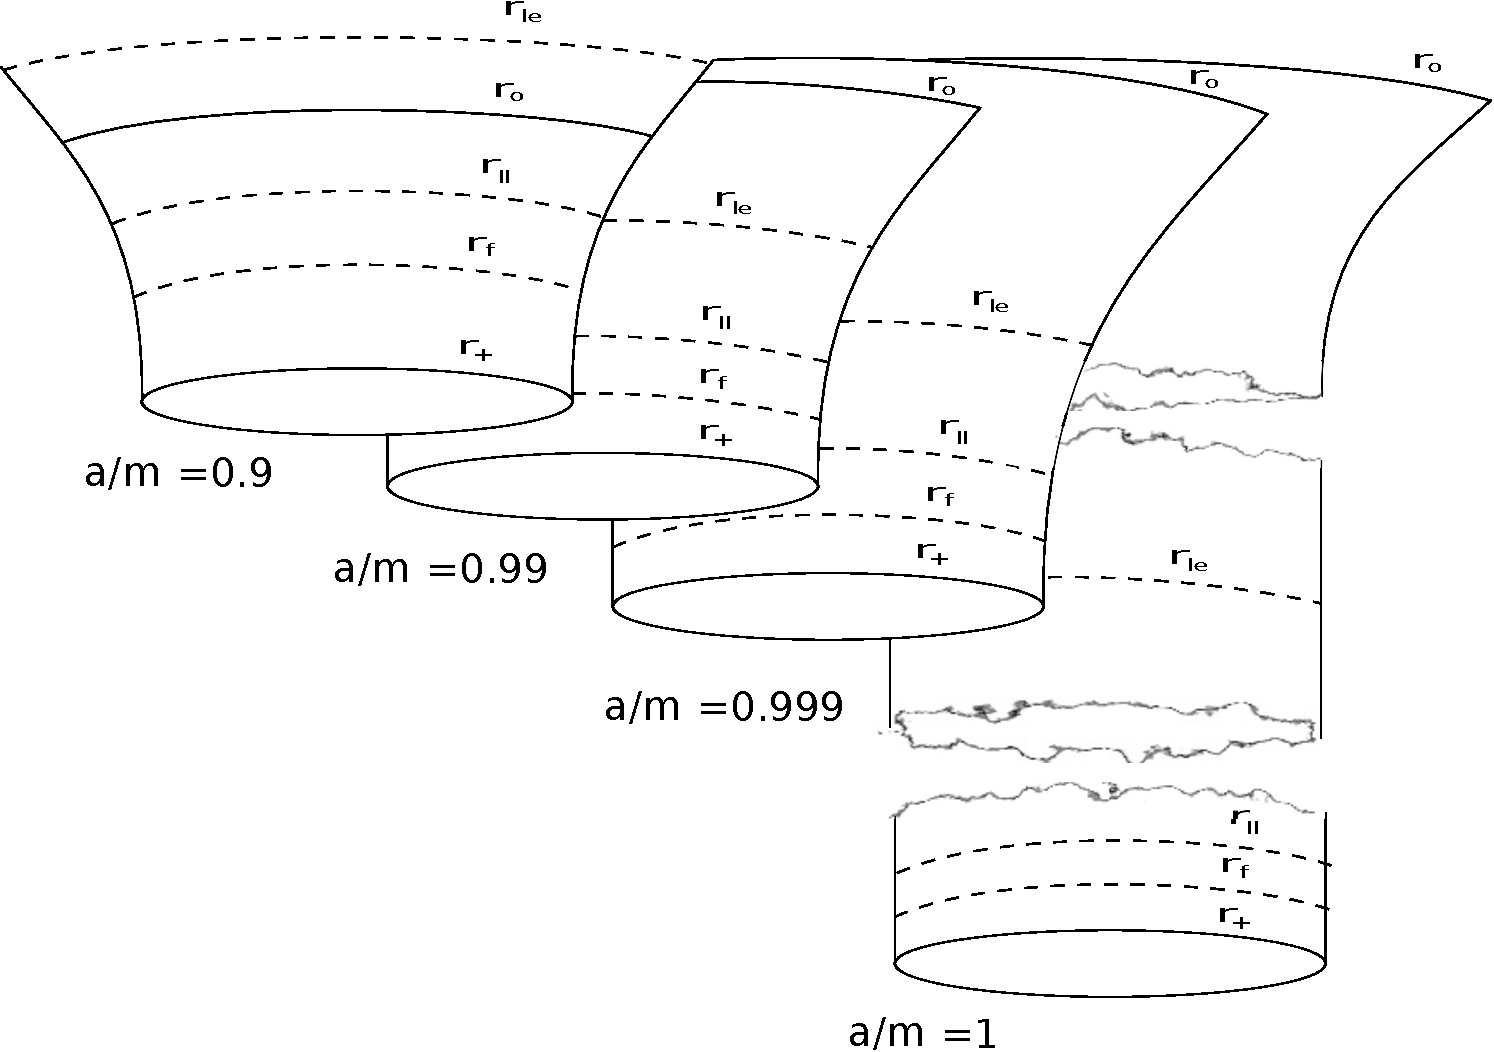
\includegraphics[height=8cm,angle=0]{fig-embedding.pdf}
%\caption{Representaci\'on de la conexi\'on causal entre \'orbitas a medida de que aumenta la velocidad angular.}
%\label{fig:tubos}
%\end{figure}


Se encuentra que \eqref{propdist} diverge cuando $r_1=r_{\rm le}$ y $r_{\rm f}=r_{\rm +}=r_{0}=r_{\rm ll}=r_{\rm f}$. Esto significa que no hay conexi\'on causal entre estos radios cuando el agujero negro es maximalmente rotante (ver figura \ref{fig:tubos}).

\subsubsection{Energ\'ia de Enlace}

La energ\'ia de enlace $E_{\rm e}$ se define como la energ\'ia necesaria para tomar la part\'icula y ponerla en el infinito (part\'icula libre con energ\'ia $E=m_0c^2$). Por lo tanto, la energ\'ia de enlace para una part\'icula de energ\'ia $E$ y masa en reposo $m_0$ es
 \begin{equation}
 \begin{aligned}
 E_{\rm e}&=E_{\rm f}-E_{\rm i}\\
 &=m_0c^2\left(1-\frac{E}{m_0c^2}\right).
 \end{aligned}
 \end{equation}
 
Para el estudio de la energ\'ia de enlace de una \'orbita circular levemente estable es conveniente reemplazar  \eqref{stable} (en el caso de la igualdad) en \eqref{Ekerr}, con lo cual se obtiene la siguiente relaci\'on
\begin{equation}
\frac{a}{m}=\mp\frac{4\sqrt{2}\left(1-\frac{E^2}{m_0^2c^4} \right)^{1/2}-\frac{2E}{m_0c^2}}{3\sqrt{3}\left(1-\frac{E^2}{m_0^2c^4} \right)}.
\end{equation}

As\'i, para part\'iculas que giran en la misma direcci\'on de giro que el agujero negro la energ\'ia decrece desde $E=(2\sqrt{2}/3)m_0c^2$ para $a=0$ hasta $E=(1/\sqrt{3})m_0c^2$ para $a=m$.\\

Para part\'iculas que giran en un sentido retr\'ogrado la energ\'ia crece desde $E=(2\sqrt{2}/3)m_0c^2$ para $a=0$ hasta $E=(5/3\sqrt{3})m_0c^2$ para $a=m$.\\

El m\'aximo valor de la energ\'ia de enlace se alcanza cuando el agujero negro es maximalmente rotante y la part\'icula gira en sentido directo, cuyo valor es $E_{\rm e}=(1-1/\sqrt{3})m_0c^2 \approx 0.423 m_0c^2$, es decir, un 42,3$\%$ de la energ\'ia en reposo de la part\'icula. Esta energ\'ia de enlace es la energ\'ia que libera la part\'icula al momento girar hacia al agujero negro a trav\'es de una serie de \'orbitas circulares. Luego, como esta energ\'ia se liber\'o en el agujero (qued\'o en aquel lugar) se puede considerar al agujero negro como una fuente de energ\'ia. Luego de pasar la \'orbita circular levemente estable, la part\'icula libera muy poca energ\'ia hasta caer dentro del agujero negro.\\

\subsection{Regi\'on de Energ\'ia Negativa}

Resolviendo la ecuaci\'on \eqref{dotr2} para $E$, se obtiene la siguiente expresi\'on:
\begin{equation}\label{energia}
\frac{E}{c}=\frac{2amL+\sqrt{L^2r^2\Delta+\left(r^3+a^2r+2ma^2\right)\left(m_0^2c^2r\Delta+\dot{r}^2r^3\right)}}{r^3+a^2r+2ma^2}.
\end{equation}

Cabe destacar la elecci\'on del signo postivo antes de la ra\'iz de \eqref{energia}, ya que en este caso al hacer $r\rightarrow \infty$ la energ\'ia es postiva ($E \geq m_0c^2$). En el caso de que $E<0$ se requiere que $L<0$ (\'orbita retr\'ograda) como se observa en \eqref{energia}, con la condici\'on de que el valor absoluto de la primera parte en el numerador de esta expresi\'on sea mayor que el valor absoluto de la segunda, o equivalentemente:
\begin{equation}\label{desigualdad}
L^2r^2\Delta+\left(r^3+a^2r+2ma^2\right)\left(m_0^2c^2r\Delta+\dot{r}^2r^3\right) < 4a^2m^2L^2.
\end{equation}

De \eqref{desigualdad}, se tiene que
\begin{equation}\label{desigualdad2}
r^2 \Delta +\left(r^3+a^2r+2ma^2\right)\left(\frac{m_0^2}{L^2}c^2r\Delta+\frac{\dot{r}^2}{L^2}r^3\right) < 4a^2m^2.
\end{equation}

Para obtener el l\'imite de la regi\'on con energ\'ia negativa se debe hacer que la parte izquierda de \eqref{desigualdad2} s\'olo tenga dependencia en la parte radial tal que $r$ tenga su mayor valor posible y se respete la desigualdad. Para lo cual se debe tener que $L>>m_0ca$ y $\dot{r} \rightarrow 0$, as\'i
\begin{equation}\label{desigualdad3}
r^2 \Delta < 4a^2m^2,
\end{equation}
donde se obtiene que el radio m\'aximo permitido es $r=r_0=2m$, es decir, el l\'imite estacionario en el plano ecuatorial. Por lo tanto las part\'iculas con energ\'ia negativa se encuentran en \'orbitas inferiores al l\'imite estacionario.\\

\subsection{Mecanismo de Penrose}

Sir Roger Penrose y R. M. Floyd explotaron  la existencia de energ\'ia negativa en un trabajo publicado en 1971 [42], donde explica c\'omo extraer energ\'ia de un agujero negro rotante, es decir, utilizar estos colosos como fuente de energ\'ia. El mec\'anismo que lleva su nombre se demuestra con el siguiente experimento pensado. Dada una part\'icula con una determinada energ\'ia $E_{\rm en}$ y una trayectoria tal que pase el l\'imite estacionario y considere que cuando se encuentre en la erg\'osfera ($r_+<r<r_0$) se divida en dos part\'iculas, una que sea capaz de salir de la erg\'osfera hacia al infinito, con una energ\'ia $E_{\rm sal}$, y otra part\'icula que tenga energ\'ia $E$ que luego sea absorbida por el agujero (que entre en el horizonte de eventos). Utilizando la conservaci\'on de energ\'ia,
\begin{equation}
E_{\rm en}=E_{\rm sal}+E,
\end{equation}
en el caso que $E<0$ se tiene que $E_{\rm sal}>E_{\rm en}$. As\'i, el hecho de existir \'orbitas en una regi\'on determinada (erg\'osfera) con energ\'ia negativa abre la posibilidad de que una part\'icula que sea observida por el agujero negro eyecte al infinito otra una energ\'ia a\'u mayor.\\

La energ\'ia con la cual sale la part\'icula es extraida de la energ\'ia rotacional del agujero negro, la cu\'al disminuye al momento que la par\'icula con energ\'ia negativa que tiene por supuesto una \'orbita retr\'ograda, es capturada.\\

De la misma forma en las ondas (electromagn\'eticas o gravitacionales) ocurre un fen\'omeno similar de amplificaci\'on de la energ\'ia donde, con un valor de la frecuencia adecuado estas ondas son dispersadas por el agujero negro rotante. Parte de la onda es absorbida y otra parte es emitida con energ\'ia mayor que la incidente. A este fen\'omeno se le llama Super Radiancia.\\

\subsubsection{L\'imite Inferior de la Velocidad Relativa}

James Maxwell Bardeen et al. en su trabajo de 1972 [43] mostraron que existe un l\'imite inferior para la velocidad relativa entre las part\'iculas (creadas de la separaci\'on de la part\'icula entrante) que se encuentran en la erg\'osfera del agujero negro para que se lleve a cabo el mecanismo de Penrose.\\

Se considera una part\'icula de masa $m_0$ y una cantidad conservada $E=cp_{\mu}\xi_{(t)}^{\mu}$ a lo largo de la geod\'esica, que se identifica con la energ\'ia, donde $\xi_{(t)}^{\mu}=(1,0,0,0)$ es el vector de Killing temporal (vector asociado a la simetr\'ia en la direcci\'on temporal de la soluci\'on de Kerr) y $p^{\mu}=m_0 u^{\mu}$ es el 4-momentum. Lo primero que se har\'a ser\'a encontrar cu\'al es rango de energ\'ia de la cantidad $E/m_0c^2$ para un punto del espacio-tiempo en general.\\

Escogiendo una tetrada ortonormal $\left(e^{\mu}_a\right)_{a=1,4}$ como base  para expresar la 4-velocidad y el vector de Killing temporal en un punto determinado, se tiene que
\begin{equation}\label{uyxi}
u^a=u^{\mu}e^a_{\mu}=(\gamma c, \gamma \vec{v}), \qquad \xi^a_{(t)}=\xi^{\mu}_{(t)}e^a_{\mu}=\left(\xi^{\hat{0}},\vec{\xi} \right).
\end{equation}
donde se satisface que $g_{\mu \nu}=\eta_{ab}e^a_{\mu}e^b_{\nu}$ con $g_{\mu \nu}$ la m\'etrica de Kerr y $\eta_{ab}$ la m\'etrica de Minkowski, donde adem\'as $\vec{v}$ es el vector velocidad de la part\'icula, $\gamma=1/\sqrt{1-\frac{v^2}{c^2}}$ y $\vec{\xi}$ es un vector en el espacio 3-dimensional.\\

De \eqref{uyxi}, el cuociente entre la energ\'ia de la part\'icula y su energ\'ia en reposo es
\begin{equation}\label{E/mu}
\frac{E}{m_0c^2}=\frac{g_{\mu \nu}u^{\mu}\xi_{(t)}^{\nu}}{c}=\frac{\eta_{ab}u^a\xi^b_{(t)}}{c}=\gamma\left(\xi^{\hat{0}}-\frac{\vec{v} \cdot \vec{\xi}}{c} \right)
\end{equation}

Una condici\'on necesaria para que \eqref{E/mu} sea un extremo es que $\vec{v}$ y $\vec{\xi}$ sean (anti)paralelos, de modo que $\vec{v} \cdot \vec{\xi}=\pm v\xi$ con $\xi=\sqrt{\vec{\xi}\cdot \vec{\xi}}$. Adem\'as, se tiene que
\begin{equation}\label{xi2}
\xi_{(t)}^2=g_{\mu \nu} \xi_{(t)}^{\mu}\xi_{(t)}^{\nu}=g_{00}=\left( 1-\frac{2mr}{\rho^2}\right)
\end{equation}
donde el valor de la norma del 4-vector es un escalar, con lo cual es independiente de las coordenadas utilizadas, en particular al utilizar las coordenadas de Kerr se obtiene \eqref{xi2}.\\

Por lo tanto, si la part\'icula se encuentra en la erg\'osfera entonces $\xi_{(t)}^{\mu}$ es un vector tipo espacio, que significa que $\xi^2_{(t)}<0$ entonces $\xi_{\hat{0}}^2-\xi^{2}<0$, con lo cual $\xi^{\hat{0}} < \xi$. As\'i, de \eqref{E/mu} se ve que todos los valores son permitidos para $E/m_0c^2$, donde el l\'imite superior se da con $v \rightarrow c$ y $\vec{v} \cdot \vec{\xi}=-v\xi$ y el inferior tambi\'en con $v \rightarrow c$ y $\vec{v} \cdot \vec{\xi}=+v\xi$. Por lo tanto,
\begin{equation}\label{condicion1}
-\infty <\frac{E}{m_0c^2}<+\infty.
\end{equation}

En el caso de estar fuera de la erg\'osfera de \eqref{xi2} se tiene que $\xi_t^{\mu}$ es tipo tiempo, con lo cual $\xi^{\hat{0}} >\xi$. Con esto el valor de la energ\'ia es siempre positivo, donde se debe determinar el l\'imite inferior del rango permitido para el couciente \eqref{E/mu}.\\

Derivando la expresi\'on \eqref{E/mu} con respecto a $v$ e igualandola a 0, se encuentra que el valor de la velocidad que extremiza el valor de la energ\'ia es:
\begin{equation}\label{v}
v=\frac{c\xi}{\xi^{\hat{0}}}.
\end{equation}

Reemplazado \eqref{v} en \eqref{E/mu}, se obtiene que el l\'imite inferior viene dado por la norma del m\'odulo del vector de Killing en el caso que es tipo tiempo $\xi_{(t)}$ (donde $\xi^2_{(t)}=\xi_{\hat{0}}^2-\xi^2$) :
\begin{equation}\label{condicion2}
\xi_{(t)}\leq  \frac{E}{m_0c^2}<+\infty.
\end{equation}

Como \eqref{condicion2} est\'a dentro del rango \eqref{condicion1}, entonces se encuentra la condici\'on general
\begin{equation}
\frac{E^{2}}{m_0^2c^4}-\xi_{(t)}^2 \geq 0.
\end{equation}

Para encontrar el l\'imite inferior para la velocidad, se debe considerar lo siguiente: Dada las \'orbitas de dos part\'iculas de masa $m_1$ y $m_2$ que se intersectan en un punto, donde las energ\'ias de cada part\'icula son $E_1$ y $E_2$, respectivamente, y con diferentes 4-velocidades, tal que la norma vector de velocidad relativo $|w|$ (velocidad de una part\'icula vista por un observador com\'ovil con la otra part\'icula) es distinto de cero.\\

Se escoge nuevamente una tetrada ortonormal como base de los 4-vectores en este punto, tal que las correspondientes 4-velocidades son
\begin{equation}
u_1^{a}=\left(\gamma c, -\gamma \vec{v} \right), \qquad u_2^{a}=\left(\gamma c, \gamma \vec{v}\right).
\end{equation}

La magnitud de la velocidad relativa $|w|$, se encuentra utilizando la f\'ormula de composici\'on de velocidades:
\begin{equation}\label{w}
|w|=\frac{2v}{1+\frac{v^2}{c^2}}.
\end{equation}

Adem\'as, de \eqref{E/mu} se tiene que
\begin{equation}\label{sistema}
\frac{E_1}{m_1c^2}=\gamma\left(\xi^{\hat{0}}+\frac{\vec{v} \cdot \vec{\xi}}{c} \right), \qquad \frac{E_2}{m_2c^2}=\gamma\left(\xi^{\hat{0}}-\frac{\vec{v} \cdot \vec{\xi}}{c} \right).
\end{equation}

Resolviendo el sistema de ecuaciones \eqref{sistema} para $\xi_{\hat{0}}^2$ y $\xi^2$, considerando que $\vec{v}\cdot \vec{\xi} \equiv v\xi \cos \eta$, donde $\eta$ es el \'angulo entre $\vec{v}$ y $\vec{\xi}$, se tiene que
\begin{equation}
\begin{aligned}
\xi_{\hat{0}}^2&=\frac{\left(\frac{E_1}{m_1c^2}+\frac{E_2}{m_2c^2} \right)^2}{4\gamma ^2},\\
\xi^2&=\frac{\left(\frac{E_1}{m_1c^2}-\frac{E_2}{m_2c^2} \right)^2}{4\frac{\gamma ^2 v^2}{c^2}\cos^2 \eta}. \\
\end{aligned}
\end{equation}

Con lo cual se tiene que
\begin{equation}
\left(\frac{E_1}{m_1c^2}-\frac{E_2}{m_2c^2} \right)^2=\left[\left(\frac{E_1}{m_1c^2}+\frac{E_2}{m_2c^2}\right)^2-4\gamma^2 \xi_{(t)}^2   \right]\frac{v^2}{c^2}\cos^2 \eta.
\end{equation}

Utilizando el hecho que $0\leq |\cos \eta| \leq 1$ se tiene que
\begin{equation}
\left(\frac{E_1}{m_1c^2}-\frac{E_2}{m_2c^2} \right)^2 \leq \left[\left(\frac{E_1}{m_1c^2}+\frac{E_2}{m_2c^2} \right)^2-4\gamma^2 \xi_{(t)}^2 \right]\frac{v^2}{c^2}.
\end{equation}

Resolviendo la \'ultima desigualdad para $v/c$ se tiene que
\begin{equation}\label{v/c}
\frac{v^2}{c^2} \geq \left[ \frac{\frac{E_1}{m_1c^2} -\frac{E_2}{m_2c^2}}{\sqrt{\frac{E_1^2}{m_{1}^{2}c^{4}}-\xi_{(t)}^2}+\sqrt{ \frac{E_2^2}{m_{2}^{2}c^{4}} -\xi_{(t)}^2}}\right]^2 .
\end{equation}

Aplicando las relaciones encontradas al caso de tener la geometr\'ia de Kerr, de \eqref{xi2} con $r \geq r_+$, encontramos
\begin{equation}
|\xi_{(t)}^2| \leq 1, \qquad  \forall \quad \theta,\varphi .
\end{equation}

Sea $E_1$ el valor de la m\'inima energ\'ia de una part\'icula que se encuentra en el m\'inimo radio en que la \'orbita circular es estable, la cual se da cuando $a \rightarrow m$ y $E_2$ tiene el valor de la energ\'ia de una part\'icula que se encuentra en el borde de la regi\'on de energ\'ia negativa
\begin{equation}
\frac{E_1}{m_1c^2}=\frac{1}{\sqrt{3}}, \qquad \frac{E_2}{m_2c^2}=0.
\end{equation}

De \eqref{v/c} se obtiene que
\begin{equation}\label{finalv/c}
\frac{v}{c} \geq 2-\sqrt{3}.
\end{equation}

Y finalmente, reemplazando \eqref{finalv/c} en \eqref{w}, se obtiene la siguiente desigualdad
\begin{equation}
|w|\geq \frac{c}{2}.
\end{equation}

As\'i, para lograr extraer energ\'ia de un agujero negro rotante la part\'icula que es capaz de salir debe acelerar a una velocidad tal que la velocidad relativa sea al menos la mitad de la velocidad de la luz, ya que bajo este requerimiento existir\'a una part\'icula en la regi\'on de energ\'ia negativa, logrando salir la part\'icula que se encuentra fuera de esta regi\'on (de energ\'ia negativa) con m\'as energ\'ia que la part\'icula entrante.\\

